% Options for packages loaded elsewhere
\PassOptionsToPackage{unicode}{hyperref}
\PassOptionsToPackage{hyphens}{url}
%
\documentclass[
]{book}
\usepackage{amsmath,amssymb}
\usepackage{lmodern}
\usepackage{iftex}
\ifPDFTeX
  \usepackage[T1]{fontenc}
  \usepackage[utf8]{inputenc}
  \usepackage{textcomp} % provide euro and other symbols
\else % if luatex or xetex
  \usepackage{unicode-math}
  \defaultfontfeatures{Scale=MatchLowercase}
  \defaultfontfeatures[\rmfamily]{Ligatures=TeX,Scale=1}
\fi
% Use upquote if available, for straight quotes in verbatim environments
\IfFileExists{upquote.sty}{\usepackage{upquote}}{}
\IfFileExists{microtype.sty}{% use microtype if available
  \usepackage[]{microtype}
  \UseMicrotypeSet[protrusion]{basicmath} % disable protrusion for tt fonts
}{}
\makeatletter
\@ifundefined{KOMAClassName}{% if non-KOMA class
  \IfFileExists{parskip.sty}{%
    \usepackage{parskip}
  }{% else
    \setlength{\parindent}{0pt}
    \setlength{\parskip}{6pt plus 2pt minus 1pt}}
}{% if KOMA class
  \KOMAoptions{parskip=half}}
\makeatother
\usepackage{xcolor}
\usepackage{color}
\usepackage{fancyvrb}
\newcommand{\VerbBar}{|}
\newcommand{\VERB}{\Verb[commandchars=\\\{\}]}
\DefineVerbatimEnvironment{Highlighting}{Verbatim}{commandchars=\\\{\}}
% Add ',fontsize=\small' for more characters per line
\usepackage{framed}
\definecolor{shadecolor}{RGB}{248,248,248}
\newenvironment{Shaded}{\begin{snugshade}}{\end{snugshade}}
\newcommand{\AlertTok}[1]{\textcolor[rgb]{0.94,0.16,0.16}{#1}}
\newcommand{\AnnotationTok}[1]{\textcolor[rgb]{0.56,0.35,0.01}{\textbf{\textit{#1}}}}
\newcommand{\AttributeTok}[1]{\textcolor[rgb]{0.77,0.63,0.00}{#1}}
\newcommand{\BaseNTok}[1]{\textcolor[rgb]{0.00,0.00,0.81}{#1}}
\newcommand{\BuiltInTok}[1]{#1}
\newcommand{\CharTok}[1]{\textcolor[rgb]{0.31,0.60,0.02}{#1}}
\newcommand{\CommentTok}[1]{\textcolor[rgb]{0.56,0.35,0.01}{\textit{#1}}}
\newcommand{\CommentVarTok}[1]{\textcolor[rgb]{0.56,0.35,0.01}{\textbf{\textit{#1}}}}
\newcommand{\ConstantTok}[1]{\textcolor[rgb]{0.00,0.00,0.00}{#1}}
\newcommand{\ControlFlowTok}[1]{\textcolor[rgb]{0.13,0.29,0.53}{\textbf{#1}}}
\newcommand{\DataTypeTok}[1]{\textcolor[rgb]{0.13,0.29,0.53}{#1}}
\newcommand{\DecValTok}[1]{\textcolor[rgb]{0.00,0.00,0.81}{#1}}
\newcommand{\DocumentationTok}[1]{\textcolor[rgb]{0.56,0.35,0.01}{\textbf{\textit{#1}}}}
\newcommand{\ErrorTok}[1]{\textcolor[rgb]{0.64,0.00,0.00}{\textbf{#1}}}
\newcommand{\ExtensionTok}[1]{#1}
\newcommand{\FloatTok}[1]{\textcolor[rgb]{0.00,0.00,0.81}{#1}}
\newcommand{\FunctionTok}[1]{\textcolor[rgb]{0.00,0.00,0.00}{#1}}
\newcommand{\ImportTok}[1]{#1}
\newcommand{\InformationTok}[1]{\textcolor[rgb]{0.56,0.35,0.01}{\textbf{\textit{#1}}}}
\newcommand{\KeywordTok}[1]{\textcolor[rgb]{0.13,0.29,0.53}{\textbf{#1}}}
\newcommand{\NormalTok}[1]{#1}
\newcommand{\OperatorTok}[1]{\textcolor[rgb]{0.81,0.36,0.00}{\textbf{#1}}}
\newcommand{\OtherTok}[1]{\textcolor[rgb]{0.56,0.35,0.01}{#1}}
\newcommand{\PreprocessorTok}[1]{\textcolor[rgb]{0.56,0.35,0.01}{\textit{#1}}}
\newcommand{\RegionMarkerTok}[1]{#1}
\newcommand{\SpecialCharTok}[1]{\textcolor[rgb]{0.00,0.00,0.00}{#1}}
\newcommand{\SpecialStringTok}[1]{\textcolor[rgb]{0.31,0.60,0.02}{#1}}
\newcommand{\StringTok}[1]{\textcolor[rgb]{0.31,0.60,0.02}{#1}}
\newcommand{\VariableTok}[1]{\textcolor[rgb]{0.00,0.00,0.00}{#1}}
\newcommand{\VerbatimStringTok}[1]{\textcolor[rgb]{0.31,0.60,0.02}{#1}}
\newcommand{\WarningTok}[1]{\textcolor[rgb]{0.56,0.35,0.01}{\textbf{\textit{#1}}}}
\usepackage{longtable,booktabs,array}
\usepackage{calc} % for calculating minipage widths
% Correct order of tables after \paragraph or \subparagraph
\usepackage{etoolbox}
\makeatletter
\patchcmd\longtable{\par}{\if@noskipsec\mbox{}\fi\par}{}{}
\makeatother
% Allow footnotes in longtable head/foot
\IfFileExists{footnotehyper.sty}{\usepackage{footnotehyper}}{\usepackage{footnote}}
\makesavenoteenv{longtable}
\usepackage{graphicx}
\makeatletter
\def\maxwidth{\ifdim\Gin@nat@width>\linewidth\linewidth\else\Gin@nat@width\fi}
\def\maxheight{\ifdim\Gin@nat@height>\textheight\textheight\else\Gin@nat@height\fi}
\makeatother
% Scale images if necessary, so that they will not overflow the page
% margins by default, and it is still possible to overwrite the defaults
% using explicit options in \includegraphics[width, height, ...]{}
\setkeys{Gin}{width=\maxwidth,height=\maxheight,keepaspectratio}
% Set default figure placement to htbp
\makeatletter
\def\fps@figure{htbp}
\makeatother
\setlength{\emergencystretch}{3em} % prevent overfull lines
\providecommand{\tightlist}{%
  \setlength{\itemsep}{0pt}\setlength{\parskip}{0pt}}
\setcounter{secnumdepth}{5}
\newlength{\cslhangindent}
\setlength{\cslhangindent}{1.5em}
\newlength{\csllabelwidth}
\setlength{\csllabelwidth}{3em}
\newlength{\cslentryspacingunit} % times entry-spacing
\setlength{\cslentryspacingunit}{\parskip}
\newenvironment{CSLReferences}[2] % #1 hanging-ident, #2 entry spacing
 {% don't indent paragraphs
  \setlength{\parindent}{0pt}
  % turn on hanging indent if param 1 is 1
  \ifodd #1
  \let\oldpar\par
  \def\par{\hangindent=\cslhangindent\oldpar}
  \fi
  % set entry spacing
  \setlength{\parskip}{#2\cslentryspacingunit}
 }%
 {}
\usepackage{calc}
\newcommand{\CSLBlock}[1]{#1\hfill\break}
\newcommand{\CSLLeftMargin}[1]{\parbox[t]{\csllabelwidth}{#1}}
\newcommand{\CSLRightInline}[1]{\parbox[t]{\linewidth - \csllabelwidth}{#1}\break}
\newcommand{\CSLIndent}[1]{\hspace{\cslhangindent}#1}
\usepackage{booktabs}
\usepackage{amsthm}
\makeatletter
\def\thm@space@setup{%
  \thm@preskip=8pt plus 2pt minus 4pt
  \thm@postskip=\thm@preskip
}
\makeatother
\ifLuaTeX
  \usepackage{selnolig}  % disable illegal ligatures
\fi
\IfFileExists{bookmark.sty}{\usepackage{bookmark}}{\usepackage{hyperref}}
\IfFileExists{xurl.sty}{\usepackage{xurl}}{} % add URL line breaks if available
\urlstyle{same} % disable monospaced font for URLs
\hypersetup{
  pdftitle={CBW pathways Workshops - example R notebooks},
  pdfauthor={Ruth Isserlin},
  hidelinks,
  pdfcreator={LaTeX via pandoc}}

\title{CBW pathways Workshops - example R notebooks}
\author{Ruth Isserlin}
\date{2023-04-24}

\begin{document}
\maketitle

{
\setcounter{tocdepth}{1}
\tableofcontents
}
\hypertarget{index}{%
\chapter{Index}\label{index}}

\hypertarget{intro}{%
\chapter{CBW Workshop example R Notebooks}\label{intro}}

Do you want to run the pathways and network analysis from R instead of doing everything mannually as demonstrated in the workshop?

Everything (almost!) that was discussed in the lectures and practicals can be done computationally through R.

We are using the \textbf{bookdown} package (\protect\hyperlink{ref-R-bookdown}{Xie 2023}) in this Workshop R Notebooks book, which was built on top of R Markdown and \textbf{knitr} (\protect\hyperlink{ref-xie2015}{Xie 2015}).

\hypertarget{setup}{%
\chapter{Setup}\label{setup}}

\hypertarget{install-r-and-rstudio}{%
\section{Install R and RStudio}\label{install-r-and-rstudio}}

As with many open source projects, \textbf{R} is a constantly evolving language with regular updates. There is a major release once a year with patch releases through out the year. Often scripts and packages will work from one release to the next (ignoring pesky warnings that a package was compiled on a previous version of R is common) but there are exceptions. Some newer packages will only work on the latest version of \textbf{R} so sometimes the choice of upgrading or not using a new package might present themselves. Often, the amount of packages and work that is need to upgrade is not realized until the process has begun. This is where docker demonstrates it most valuable features. You can create a new instance based on the latest release of \textbf{R} and all your needed packages without having to change any of your current settings.

In order to use these notebooks supplied here you need to have:

\begin{itemize}
\tightlist
\item
  \textbf{R} installed on your computer and
\item
  a list of packages. (including BiocManager, BiomaRt, gprofiler2, GSA)
\end{itemize}

Each notebook in this set will check for the required packages and install them if they are missing so at the base level you need to just have \textbf{R} installed.

There are many different ways you can use and setup \textbf{R}.

\begin{enumerate}
\def\labelenumi{\arabic{enumi}.}
\tightlist
\item
  By simply installing \textbf{R} you can use it directly but
\item
  it is highly recommended that you also install and use \href{https://rstudio.com/products/rstudio/download/}{RStudio} which is an Integrate development environment (IDE) for \textbf{R}. You cannot just download RStudio and use it. It requires an installation of \textbf{R}.
\end{enumerate}

You don't need to install R and RStudio though. You can also use \textbf{R} and RStudio through docker. \textbf{I highly recommend using docker instead}

\hypertarget{docker-optional}{%
\section{Docker {[}Optional{]}}\label{docker-optional}}

Changing versions and environments are a continuing struggle with bioinformatics pipelines and computational pipelines in general. An analysis written and performed a year ago might not run or produce the same results when it is run today. Recording package and system versions or not updating certain packages rarely work in the long run.

One the best solutions to reproducibility issues is containing your workflow or pipeline in its own coding environment where everything from the operating system, programs and packages are defined and can be built from a set of given instructions. There are many systems that offer this type of control including:

\begin{itemize}
\tightlist
\item
  \href{https://www.docker.com/}{Docker}.
\item
  \href{https://sylabs.io/}{Singularity}
\end{itemize}

``A container is a standard unit of software that packages up code and all its dependencies so the application runs quickly and reliably from one computing environment to another.'' (\protect\hyperlink{ref-docker}{{``What Is a Container?''} n.d.})

\textbf{Why are containers great for Bioiformatics?}

\begin{itemize}
\tightlist
\item
  allows you to create environments to run bioinformatis pipelines.
\item
  create a consistent environment to use for your pipelines.
\item
  test modifications to the pipeline without disrupting your current set up.
\item
  Coming back to an analysis years later and there is no need to install older versions of packages or programming languages. Simply create a container and re-run.
\end{itemize}

\hypertarget{install-docker}{%
\section{Install Docker}\label{install-docker}}

\begin{enumerate}
\def\labelenumi{\arabic{enumi}.}
\tightlist
\item
  Download and install \href{https://www.docker.com/products/docker-desktop}{docker desktop}.
\item
  Follow slightly different instructions for Windows or MacOS/Linux
\end{enumerate}

\hypertarget{windows}{%
\subsection{Windows}\label{windows}}

\begin{itemize}
\tightlist
\item
  it might prompt you to install additional updates (for example - \url{https://docs.Microsoft.com/en-us/windows/wsl/install-win10\#step-4---download-the-linux-kernel-update-package}) and require multiple restarts of your system or docker.
\item
  launch docker desktop app.
\item
  Open windows Power shell
\item
  navigate to directory on your system where you plan on keeping all your code. For example: C:\textbackslash USERS\textbackslash risserlin\textbackslash cbw\_workshop\_code
\item
  Run the following command: (the only difference with the windows command is the way the current directory is written. \$\{PWD\} instead of "\$(pwd)")
\end{itemize}

\begin{Shaded}
\begin{Highlighting}[]
\NormalTok{docker run }\SpecialCharTok{{-}}\NormalTok{e PASSWORD}\OtherTok{=}\NormalTok{changeit }\SpecialCharTok{{-}{-}}\NormalTok{rm \textbackslash{}}
  \SpecialCharTok{{-}}\NormalTok{v }\SpecialCharTok{$}\NormalTok{\{PWD\}}\SpecialCharTok{:}\ErrorTok{/}\NormalTok{home}\SpecialCharTok{/}\NormalTok{rstudio}\SpecialCharTok{/}\NormalTok{projects }\SpecialCharTok{{-}}\NormalTok{p }\DecValTok{8787}\SpecialCharTok{:}\DecValTok{8787}\NormalTok{ \textbackslash{}}
\NormalTok{  risserlin}\SpecialCharTok{/}\NormalTok{workshop\_base\_image}
\end{Highlighting}
\end{Shaded}

\begin{itemize}
\tightlist
\item
  Windows defender firewall might pop up with warning. Click on \emph{Allow access}.
\item
  In docker desktop you see all containers you are running and easily manage them.
\end{itemize}

\hypertarget{macos-linux}{%
\subsection{MacOS / Linux}\label{macos-linux}}

\begin{itemize}
\tightlist
\item
  Open Terminal
\item
  navigate to directory on your system where you plan on keeping all your code. For example: /Users/risserlin/bcb420\_code
\item
  Run the following command: (the only difference with the windows command is the way the current directory is written. \$\{PWD\} instead of "\$(pwd)")
\end{itemize}

\begin{Shaded}
\begin{Highlighting}[]
\NormalTok{docker run }\SpecialCharTok{{-}}\NormalTok{e PASSWORD}\OtherTok{=}\NormalTok{changeit }\SpecialCharTok{{-}{-}}\NormalTok{rm \textbackslash{}}
  \SpecialCharTok{{-}}\NormalTok{v }\StringTok{"$(pwd)"}\SpecialCharTok{:}\ErrorTok{/}\NormalTok{home}\SpecialCharTok{/}\NormalTok{rstudio}\SpecialCharTok{/}\NormalTok{projects }\SpecialCharTok{{-}}\NormalTok{p }\DecValTok{8787}\SpecialCharTok{:}\DecValTok{8787}\NormalTok{ \textbackslash{}}
  \SpecialCharTok{{-}{-}}\NormalTok{add}\SpecialCharTok{{-}}\NormalTok{host }\StringTok{"localhost:My.IP.address"}
\NormalTok{  risserlin}\SpecialCharTok{/}\NormalTok{workshop\_base\_image}
\end{Highlighting}
\end{Shaded}

\hypertarget{run-gprofiler-from-r}{%
\chapter{Run g:profiler from R}\label{run-gprofiler-from-r}}

\hypertarget{initialize-variables-and-libraries}{%
\section{Initialize variables and libraries}\label{initialize-variables-and-libraries}}

Detailed instructions on how to run \href{https://biit.cs.ut.ee/gprofiler/gost}{g:Profiler} programmatically from R

The parameters are set manually here but if you want to run the script from the command line then you can update the notebook to pull the parameters from the command line given arguments by updating each variable below to pull the values from the paramters - for example:

\begin{itemize}
\tightlist
\item
  variable \textless- params\$parameter\_name
\end{itemize}

For more details see - \href{https://bookdown.org/yihui/rmarkdown/params-declare.html}{defining and using parameters} and \href{https://bookdown.org/yihui/rmarkdown/params-knit.html}{Knitting with parameters}

\begin{Shaded}
\begin{Highlighting}[]
\CommentTok{\#where to put all the generated files}
\NormalTok{working\_dir }\OtherTok{\textless{}{-}} \StringTok{"./generated\_data/g\_profiler"}

\CommentTok{\# where to find the data files needed to run the analysis}
\NormalTok{data\_dir }\OtherTok{\textless{}{-}}  \StringTok{"./data"}

\CommentTok{\# File name containing the list of genes to be used for analysis}
\NormalTok{genelist\_file }\OtherTok{\textless{}{-}} \StringTok{"Supplementary\_Table1\_Cancer\_drivers.txt"}

\CommentTok{\# default max size of the genesets for example {-}  250.  For this example we}
\CommentTok{\# will be varying this parameter}
\NormalTok{max\_gs\_size }\OtherTok{\textless{}{-}} \DecValTok{250}

\CommentTok{\# default min size of the genesets for example {-}  3}
\NormalTok{min\_gs\_size }\OtherTok{\textless{}{-}} \DecValTok{3}

\CommentTok{\#min intersection between your genelist and the geneset {-} for example 3}
\NormalTok{min\_intersection }\OtherTok{\textless{}{-}} \DecValTok{3}

\CommentTok{\# organism parameter used for g:profiler.  }
\CommentTok{\# First letter of first word in species name followed by }
\CommentTok{\# the second word for example {-} hsapiens}
\NormalTok{organism }\OtherTok{\textless{}{-}} \StringTok{"hsapiens"}
\end{Highlighting}
\end{Shaded}

\begin{Shaded}
\begin{Highlighting}[]
\CommentTok{\#use library}
\FunctionTok{tryCatch}\NormalTok{(}\AttributeTok{expr =}\NormalTok{ \{ }\FunctionTok{library}\NormalTok{(}\StringTok{"gprofiler2"}\NormalTok{)\}, }
         \AttributeTok{error =} \ControlFlowTok{function}\NormalTok{(e) \{ }
           \FunctionTok{install.packages}\NormalTok{(}\StringTok{"gprofiler2"}\NormalTok{)\}, }
         \AttributeTok{finally =} \FunctionTok{library}\NormalTok{(}\StringTok{"gprofiler2"}\NormalTok{))}

\FunctionTok{tryCatch}\NormalTok{(}\AttributeTok{expr =}\NormalTok{ \{ }\FunctionTok{library}\NormalTok{(}\StringTok{"GSA"}\NormalTok{)\}, }
         \AttributeTok{error =} \ControlFlowTok{function}\NormalTok{(e) \{ }
           \FunctionTok{install.packages}\NormalTok{(}\StringTok{"GSA"}\NormalTok{)\}, }
         \AttributeTok{finally =} \FunctionTok{library}\NormalTok{(}\StringTok{"GSA"}\NormalTok{))}
\end{Highlighting}
\end{Shaded}

Create or set a directory to store all the generatd results

\begin{Shaded}
\begin{Highlighting}[]
\ControlFlowTok{if}\NormalTok{(}\SpecialCharTok{!}\FunctionTok{dir.exists}\NormalTok{(params}\SpecialCharTok{$}\NormalTok{working\_dir))\{}
  \FunctionTok{dir.create}\NormalTok{(params}\SpecialCharTok{$}\NormalTok{working\_dir)}
\NormalTok{\}}
\end{Highlighting}
\end{Shaded}

\hypertarget{load-in-query-set}{%
\section{Load in Query set}\label{load-in-query-set}}

Load in the set of genes that we will be running g:profiler with

\begin{Shaded}
\begin{Highlighting}[]
 \CommentTok{\#load in the file}
\NormalTok{    current\_genelist }\OtherTok{\textless{}{-}} \FunctionTok{read.table}\NormalTok{(}\AttributeTok{file =} 
                                     \FunctionTok{file.path}\NormalTok{(data\_dir, genelist\_file),}
                                   \AttributeTok{header =} \ConstantTok{FALSE}\NormalTok{,}
                                   \AttributeTok{sep =} \StringTok{"}\SpecialCharTok{\textbackslash{}t}\StringTok{"}\NormalTok{, }\AttributeTok{quote =} \StringTok{""}\NormalTok{,}
                                   \AttributeTok{stringsAsFactors =} \ConstantTok{FALSE}\NormalTok{)}

\NormalTok{  query\_set }\OtherTok{\textless{}{-}}\NormalTok{ current\_genelist}\SpecialCharTok{$}\NormalTok{V1}
\end{Highlighting}
\end{Shaded}

With regards to pathway sets there are two options when using \href{https://biit.cs.ut.ee/gprofiler/gost}{g:Profiler} -

\begin{itemize}
\tightlist
\item
  Use the genesets that are supplied by \href{https://biit.cs.ut.ee/gprofiler/gost}{g:Profiler}
\item
  Upload your own genesets.
\end{itemize}

The most common reasons for supplying your own genesets is the ability to use up to date annotations or in-house annotations that might not be available in the public sphere yet. One of the greatest features of \href{https://biit.cs.ut.ee/gprofiler/gost}{g:Profiler} is that it is updated on a regular basis and most of the previous versions are available online ont the \href{https://biit.cs.ut.ee/gprofiler/page/archives}{gprofiler archive}.

The \href{https://biit.cs.ut.ee/gprofiler/page/r}{gprofielr2} -\href{https://biit.cs.ut.ee/gprofiler/gost}{g:Profiler} R implementation is a wrapper for the web version. You require an internet connection to get enrichment results.

\hypertarget{run-gprofiler-with-supplied-genesets}{%
\section{Run g:profiler with supplied genesets}\label{run-gprofiler-with-supplied-genesets}}

For detailed descriptions of all the parameters that can be specified for the gost g:profiler function see -\href{https://rdrr.io/cran/gprofiler2/man/gost.html}{here}

For this query we are specifying -

\begin{itemize}
\tightlist
\item
  query - the set of genes of interest, as loaded in from the Supplementary\_Table1\_Cancer\_drivers.txt file.
\item
  significant - set to FALSE because we want g:Profiler to return all the results not just the ones that it deems significant by its perdetermined threshold.
\item
  ordered\_query - set to TRUE because for this set of genes they are ordered in order of their significance
\item
  correction\_method - set to fdr. by default g:Profiler uses g:Scs
\item
  organism - set to ``hsapiens'' for homo sapiens. Organism names are constructed by concatenating the first letter of the name and the family name (according to gprofiler2 documentation)
\item
  source - the geneset source databases to use for the analysis. We recommend using GO biological process (\url{GO:BP}), WikiPathways (WP) and Reactome (Reac) but there are additional sources you can add (GO molecular function or cellular component(\url{GO:MF}, \url{GO:CC}), KEGG, transcription factors (TF), microRNA targets (MIRNA), corum complexes (CORUM), Human protein atlas (HPA),Human phenotype ontology (HP) )
\end{itemize}

\begin{Shaded}
\begin{Highlighting}[]
\NormalTok{gprofiler\_results }\OtherTok{\textless{}{-}} \FunctionTok{gost}\NormalTok{(}\AttributeTok{query =}\NormalTok{ query\_set ,}
                          \AttributeTok{significant=}\ConstantTok{FALSE}\NormalTok{,}
                          \AttributeTok{ordered\_query =} \ConstantTok{TRUE}\NormalTok{,}
                          \AttributeTok{exclude\_iea=}\ConstantTok{FALSE}\NormalTok{,}
                          \AttributeTok{correction\_method =} \StringTok{"fdr"}\NormalTok{,}
                          \AttributeTok{organism =}\NormalTok{ organism,}
                          \AttributeTok{source =} \FunctionTok{c}\NormalTok{(}\StringTok{"REAC"}\NormalTok{,}\StringTok{"WP"}\NormalTok{,}\StringTok{"GO:BP"}\NormalTok{))}
\end{Highlighting}
\end{Shaded}

\begin{Shaded}
\begin{Highlighting}[]
 \CommentTok{\#get the gprofiler results table}
\NormalTok{enrichment\_results }\OtherTok{\textless{}{-}}\NormalTok{ gprofiler\_results}\SpecialCharTok{$}\NormalTok{result}
    
\NormalTok{enrichment\_results[}\DecValTok{1}\SpecialCharTok{:}\DecValTok{5}\NormalTok{,]}
\end{Highlighting}
\end{Shaded}

\begin{verbatim}
##     query significant      p_value term_size query_size intersection_size
## 1 query_1        TRUE 9.272751e-39      5493        121               103
## 2 query_1        TRUE 1.694623e-36      5836        121               103
## 3 query_1        TRUE 1.276992e-35      5662        121               101
## 4 query_1        TRUE 4.128404e-35      2976        121                79
## 5 query_1        TRUE 1.198524e-34      3131        121                80
##   precision     recall    term_id source
## 1 0.8512397 0.01875114 GO:0031323  GO:BP
## 2 0.8512397 0.01764907 GO:0080090  GO:BP
## 3 0.8347107 0.01783822 GO:0051171  GO:BP
## 4 0.6528926 0.02654570 GO:0031325  GO:BP
## 5 0.6611570 0.02555094 GO:0051173  GO:BP
##                                                    term_name
## 1                   regulation of cellular metabolic process
## 2                    regulation of primary metabolic process
## 3          regulation of nitrogen compound metabolic process
## 4          positive regulation of cellular metabolic process
## 5 positive regulation of nitrogen compound metabolic process
##   effective_domain_size source_order
## 1                 21110         7510
## 2                 21110        18790
## 3                 21110        14316
## 4                 21110         7512
## 5                 21110        14318
##                                          parents
## 1             GO:0019222, GO:0044237, GO:0050794
## 2                         GO:0019222, GO:0044238
## 3                         GO:0006807, GO:0019222
## 4 GO:0009893, GO:0031323, GO:0044237, GO:0048522
## 5             GO:0006807, GO:0009893, GO:0051171
\end{verbatim}

\hypertarget{download-and-load-gprofiler-geneset-file}{%
\section{Download and load g:profiler geneset file}\label{download-and-load-gprofiler-geneset-file}}

In order to create a proper Generic enrichment results file we will need a copy of the gmt file used by g:Profiler. (also to create an Enrichment map).

Download the gmt file used for this analysis from g:profiler

\begin{Shaded}
\begin{Highlighting}[]
\CommentTok{\#the link to the gmt file is static no matter what version}
\NormalTok{gprofiler\_gmt\_url }\OtherTok{\textless{}{-}} 
  \StringTok{"https://biit.cs.ut.ee/gprofiler/static/gprofiler\_full\_hsapiens.name.gmt"}

\CommentTok{\#get version info gprofiler as the gmt file is always associated with }
\CommentTok{\# a specific version of g:profiler}
\NormalTok{gprofiler\_version }\OtherTok{\textless{}{-}} \FunctionTok{get\_version\_info}\NormalTok{(}\AttributeTok{organism=}\NormalTok{organism)}

\NormalTok{gprofiler\_gmt\_filename }\OtherTok{\textless{}{-}} \FunctionTok{file.path}\NormalTok{(working\_dir,}
                                  \FunctionTok{paste}\NormalTok{(}\StringTok{"gprofiler\_full"}\NormalTok{, organism,}
\NormalTok{                                    gprofiler\_version}\SpecialCharTok{$}\NormalTok{gprofiler\_version,}\AttributeTok{sep=}\StringTok{"\_"}\NormalTok{,}
                                    \StringTok{".name.gmt"}\NormalTok{))}

\ControlFlowTok{if}\NormalTok{(}\SpecialCharTok{!}\FunctionTok{file.exists}\NormalTok{(gprofiler\_gmt\_filename))\{}
  \FunctionTok{download.file}\NormalTok{(}\AttributeTok{url =}\NormalTok{ gprofiler\_gmt\_url, }
              \AttributeTok{destfile =}\NormalTok{ gprofiler\_gmt\_filename)}
\NormalTok{\}}
\end{Highlighting}
\end{Shaded}

To create a proper Generic enrichmentMap results file we need to include the list of genes that are associated with each geneset. To do that we need to know what genes are associated with each set and filter them by our query set. Load in the geneset definitions from the gmt file we just downloaded from g:profiler site.

\begin{Shaded}
\begin{Highlighting}[]
\CommentTok{\#load in the g:profiler geneset file}
\NormalTok{capt\_output }\OtherTok{\textless{}{-}} \FunctionTok{capture.output}\NormalTok{(genesets\_gprofiler }\OtherTok{\textless{}{-}} \FunctionTok{GSA.read.gmt}\NormalTok{(}
                                      \AttributeTok{filename =}\NormalTok{ gprofiler\_gmt\_filename))}

\FunctionTok{names}\NormalTok{(genesets\_gprofiler}\SpecialCharTok{$}\NormalTok{genesets) }\OtherTok{\textless{}{-}}\NormalTok{ genesets\_gprofiler}\SpecialCharTok{$}\NormalTok{geneset.names}
\end{Highlighting}
\end{Shaded}

For the next module the name of the gmt file is - gprofiler\_full\_hsapiens.name.gmt but it is important to preserve the database version so in the future when we revisit these results for publication or results verfication we have the exact version used. Instead of creating a copy of the file (which can be pretty large) create a symbolic link to the file with the generic name.

\begin{Shaded}
\begin{Highlighting}[]
\CommentTok{\#file.exists does not work for a symbolic link on my computer for some reason}
\CommentTok{\# list the files in the directory and check if the symbolic link is there}
\CommentTok{\#if(file.exists(file.path(working\_dir, "gprofiler\_full\_hsapiens.name.gmt")))\{}
\ControlFlowTok{if}\NormalTok{(}\FunctionTok{length}\NormalTok{(}\FunctionTok{grep}\NormalTok{(}\AttributeTok{x =} \FunctionTok{list.files}\NormalTok{(}\FunctionTok{file.path}\NormalTok{(working\_dir)), }
              \AttributeTok{pattern =} \StringTok{"gprofiler\_full\_hsapiens.name.gmt"}\NormalTok{,}
              \AttributeTok{fixed =} \ConstantTok{TRUE}\NormalTok{) }\SpecialCharTok{\textgreater{}} \DecValTok{0}\NormalTok{ ))\{}

  \FunctionTok{file.remove}\NormalTok{(}\FunctionTok{file.path}\NormalTok{(working\_dir, }\StringTok{"gprofiler\_full\_hsapiens.name.gmt"}\NormalTok{))}
\NormalTok{\}}
\end{Highlighting}
\end{Shaded}

\begin{verbatim}
## [1] TRUE
\end{verbatim}

\begin{Shaded}
\begin{Highlighting}[]
\FunctionTok{file.symlink}\NormalTok{( gprofiler\_gmt\_filename,}\FunctionTok{file.path}\NormalTok{(working\_dir, }
                                   \StringTok{"gprofiler\_full\_hsapiens.name.gmt"}\NormalTok{))}
\end{Highlighting}
\end{Shaded}

\begin{verbatim}
## [1] TRUE
\end{verbatim}

\begin{Shaded}
\begin{Highlighting}[]
\CommentTok{\# Given:}
\CommentTok{\# query\_genes {-} genes used for enrichment analysis (or as query)}
\CommentTok{\#}
\CommentTok{\# returns {-} the genes that overlap with the query set and part of the given}
\CommentTok{\#           genesets}
\NormalTok{getGenesetGenes }\OtherTok{\textless{}{-}} \ControlFlowTok{function}\NormalTok{(query\_genes, subset\_genesets)\{}
\NormalTok{  genes }\OtherTok{\textless{}{-}} \FunctionTok{lapply}\NormalTok{(subset\_genesets,}\AttributeTok{FUN=}\ControlFlowTok{function}\NormalTok{(x)\{}\FunctionTok{intersect}\NormalTok{(x,query\_genes)\})}
  
  \CommentTok{\# For each of the genes collapse to the comma separate text}
\NormalTok{  genes\_collapsed }\OtherTok{\textless{}{-}} \FunctionTok{unlist}\NormalTok{(}\FunctionTok{lapply}\NormalTok{(genes,}\AttributeTok{FUN=}\ControlFlowTok{function}\NormalTok{(x)\{}
                                                \FunctionTok{paste}\NormalTok{(x,}\AttributeTok{collapse =} \StringTok{","}\NormalTok{)\}))}
  
\NormalTok{  genes\_collapsed\_df }\OtherTok{\textless{}{-}} \FunctionTok{data.frame}\NormalTok{(}\AttributeTok{term\_id =} \FunctionTok{names}\NormalTok{(genes), }
                            \AttributeTok{genes =}\NormalTok{ genes\_collapsed,}\AttributeTok{stringsAsFactors =} \ConstantTok{FALSE}\NormalTok{)}
  
  \FunctionTok{return}\NormalTok{(genes\_collapsed\_df)}
\NormalTok{\}}
\end{Highlighting}
\end{Shaded}

\hypertarget{filter-results-by-geneset-size}{%
\section{Filter results by geneset size}\label{filter-results-by-geneset-size}}

Filter the table to include just the columns that are required for the generic enrichment map file results \href{https://enrichmentmap.readthedocs.io/en/latest/FileFormats.html\#generic-results-files}{GEM}. Restrict the results to just the ones that have at least min\_gs\_size and less than max\_gs\_size terms and min\_intersection size include only the term\_id, term\_name, p\_value (and p\_value again because the p\_value is actually the corrected p-value. The output file does not contain the nominal p\_value. For down stream analysis though it is expected to have both a p-value and a q-value so just duplicate the q-value as both p-value and q-value)

Vary the thresholds for max\_gs\_size just as we did in Module 2 lab -

\begin{itemize}
\item
  min\_gs\_size = 3
\item
  max\_gs\_size = 10000
\item
  max\_gs\_size = 1000
\item
  max\_gs\_size = 250
\end{itemize}

\begin{Shaded}
\begin{Highlighting}[]
\CommentTok{\# filer by params defined above}
\CommentTok{\# by default we have set the max and min gs size to 250 and 3, respectively.}
\NormalTok{enrichment\_results\_mxgssize\_250\_min\_3 }\OtherTok{\textless{}{-}} 
                        \FunctionTok{subset}\NormalTok{(enrichment\_results,term\_size }\SpecialCharTok{\textgreater{}=}\NormalTok{ min\_gs\_size }\SpecialCharTok{\&} 
\NormalTok{                                   term\_size }\SpecialCharTok{\textless{}=}\NormalTok{ max\_gs\_size }\SpecialCharTok{\&} 
\NormalTok{                                   intersection\_size }\SpecialCharTok{\textgreater{}=}\NormalTok{ min\_intersection , }
                                 \AttributeTok{select =} \FunctionTok{c}\NormalTok{(term\_id,term\_name,p\_value,p\_value ))}

\NormalTok{enrichment\_results\_mxgssize\_1000\_min\_3 }\OtherTok{\textless{}{-}} 
                        \FunctionTok{subset}\NormalTok{(enrichment\_results,term\_size }\SpecialCharTok{\textgreater{}=}\NormalTok{ min\_gs\_size }\SpecialCharTok{\&} 
\NormalTok{                                   term\_size }\SpecialCharTok{\textless{}=} \DecValTok{1000} \SpecialCharTok{\&} 
\NormalTok{                                   intersection\_size }\SpecialCharTok{\textgreater{}=}\NormalTok{ min\_intersection , }
                                 \AttributeTok{select =} \FunctionTok{c}\NormalTok{(term\_id,term\_name,p\_value,p\_value ))}

\NormalTok{enrichment\_results\_mxgssize\_10000\_min\_3 }\OtherTok{\textless{}{-}} 
                        \FunctionTok{subset}\NormalTok{(enrichment\_results,term\_size }\SpecialCharTok{\textgreater{}=}\NormalTok{ min\_gs\_size }\SpecialCharTok{\&} 
\NormalTok{                                   term\_size }\SpecialCharTok{\textless{}=} \DecValTok{10000} \SpecialCharTok{\&} 
\NormalTok{                                   intersection\_size }\SpecialCharTok{\textgreater{}=}\NormalTok{ min\_intersection , }
                                 \AttributeTok{select =} \FunctionTok{c}\NormalTok{(term\_id,term\_name,p\_value,p\_value ))}
\end{Highlighting}
\end{Shaded}

\hypertarget{create-an-output-file-of-the-results---generic-enrichment-map-file-from-gprofiler-gmt}{%
\section{Create an output file of the results - Generic enrichment Map file from g:profiler gmt}\label{create-an-output-file-of-the-results---generic-enrichment-map-file-from-gprofiler-gmt}}

The file requires -

\begin{itemize}
\tightlist
\item
  name
\item
  description
\item
  p-value
\item
  q-value
\item
  phenotyp
\item
  list of genes (overlap of query set and original geneset)
\end{itemize}

The list of genes needs to be calculated using the gmt file and original query set. For each geneset found in the result find the overlap between the set of genes that are a part of the geneset and the query set.

\begin{Shaded}
\begin{Highlighting}[]
\CommentTok{\# Given:}
\CommentTok{\# gprofiler\_results {-} results form g\_profiler R function (filtered by desired)}
\CommentTok{\# parameters}
\CommentTok{\# gs {-} genes associated with each geneset, loaded in from a gmt file. }
\CommentTok{\#}
\CommentTok{\# returns {-} the properly formatted GEM file results}
\CommentTok{\#}
\NormalTok{createGEMformat }\OtherTok{\textless{}{-}} \ControlFlowTok{function}\NormalTok{(results, gs, query\_genes)\{}

  \ControlFlowTok{if}\NormalTok{(}\FunctionTok{nrow}\NormalTok{(results) }\SpecialCharTok{\textgreater{}}\DecValTok{0}\NormalTok{)\{    }

           \CommentTok{\#add phenotype to the results}
\NormalTok{          formatted\_results }\OtherTok{\textless{}{-}} \FunctionTok{cbind}\NormalTok{(results,}\DecValTok{1}\NormalTok{)}
          
          \CommentTok{\# Add the genes to the genesets}
\NormalTok{          subset\_genesets }\OtherTok{\textless{}{-}}\NormalTok{ gs}\SpecialCharTok{$}\NormalTok{genesets[}
            \FunctionTok{which}\NormalTok{(gs}\SpecialCharTok{$}\NormalTok{geneset.names }
                  \SpecialCharTok{\%in\%}\NormalTok{ results}\SpecialCharTok{$}\NormalTok{term\_id)]}
          
\NormalTok{          genes }\OtherTok{\textless{}{-}} \FunctionTok{getGenesetGenes}\NormalTok{(query\_genes, subset\_genesets)}
          
\NormalTok{          formatted\_results }\OtherTok{\textless{}{-}} \FunctionTok{merge}\NormalTok{(formatted\_results,genes,}\AttributeTok{by.x=}\DecValTok{1}\NormalTok{, }\AttributeTok{by.y=}\DecValTok{1}\NormalTok{)}
          
          \FunctionTok{colnames}\NormalTok{(formatted\_results) }\OtherTok{\textless{}{-}} \FunctionTok{c}\NormalTok{(}\StringTok{"name"}\NormalTok{,}\StringTok{"description"}\NormalTok{,}\StringTok{"p{-}value"}\NormalTok{,}
                                           \StringTok{"q{-}value"}\NormalTok{,}\StringTok{"phenotype"}\NormalTok{,}\StringTok{"genes"}\NormalTok{)}
          
\NormalTok{  \}}
  \FunctionTok{return}\NormalTok{(formatted\_results)}
\NormalTok{\}}
\end{Highlighting}
\end{Shaded}

\begin{Shaded}
\begin{Highlighting}[]
\NormalTok{enrichment\_results\_mxgssize\_10000\_min\_3\_GEMfile }\OtherTok{\textless{}{-}} \FunctionTok{createGEMformat}\NormalTok{(}
\NormalTok{  enrichment\_results\_mxgssize\_10000\_min\_3, genesets\_gprofiler, query\_set)}

\NormalTok{enrichment\_results\_mxgssize\_1000\_min\_3\_GEMfile }\OtherTok{\textless{}{-}} \FunctionTok{createGEMformat}\NormalTok{(}
\NormalTok{  enrichment\_results\_mxgssize\_1000\_min\_3, genesets\_gprofiler, query\_set)}

\NormalTok{enrichment\_results\_mxgssize\_250\_min\_3\_GEMfile }\OtherTok{\textless{}{-}} \FunctionTok{createGEMformat}\NormalTok{(}
\NormalTok{  enrichment\_results\_mxgssize\_250\_min\_3, genesets\_gprofiler, query\_set)}
\end{Highlighting}
\end{Shaded}

Output each of the above filtered files

\begin{Shaded}
\begin{Highlighting}[]
\CommentTok{\#output the enrichment map file}
\FunctionTok{write.table}\NormalTok{(enrichment\_results\_mxgssize\_10000\_min\_3\_GEMfile, }
            \AttributeTok{file =} \FunctionTok{file.path}\NormalTok{(working\_dir, }
                \StringTok{"gProfiler\_hsapiens\_lab2\_results\_GEM\_maxterm10000.txt"}\NormalTok{),}
            \AttributeTok{row.names =} \ConstantTok{FALSE}\NormalTok{, }
            \AttributeTok{col.names =} \ConstantTok{TRUE}\NormalTok{,}
            \AttributeTok{quote =} \ConstantTok{FALSE}\NormalTok{)}

\CommentTok{\#output the enrichment map file}
\FunctionTok{write.table}\NormalTok{(enrichment\_results\_mxgssize\_1000\_min\_3\_GEMfile, }
            \AttributeTok{file =} \FunctionTok{file.path}\NormalTok{(working\_dir, }
                \StringTok{"gProfiler\_hsapiens\_lab2\_results\_GEM\_maxterm1000.txt"}\NormalTok{),}
            \AttributeTok{row.names =} \ConstantTok{FALSE}\NormalTok{, }
            \AttributeTok{col.names =} \ConstantTok{TRUE}\NormalTok{,}
            \AttributeTok{quote =} \ConstantTok{FALSE}\NormalTok{)}

\CommentTok{\#output the enrichment map file}
\FunctionTok{write.table}\NormalTok{(enrichment\_results\_mxgssize\_250\_min\_3\_GEMfile, }
            \AttributeTok{file =} \FunctionTok{file.path}\NormalTok{(working\_dir, }
                \StringTok{"gProfiler\_hsapiens\_lab2\_results\_GEM\_maxterm250.txt"}\NormalTok{),}
            \AttributeTok{row.names =} \ConstantTok{FALSE}\NormalTok{, }
            \AttributeTok{col.names =} \ConstantTok{TRUE}\NormalTok{,}
            \AttributeTok{quote =} \ConstantTok{FALSE}\NormalTok{)}
\end{Highlighting}
\end{Shaded}

\hypertarget{run-gprofiler-with-your-own-genesets-example-using-baderlab-genesets}{%
\section{Run g:profiler with your own genesets (example using BaderLab genesets)}\label{run-gprofiler-with-your-own-genesets-example-using-baderlab-genesets}}

\hypertarget{download-and-load-bader-lab-geneset-file}{%
\section{Download and load Bader lab geneset file}\label{download-and-load-bader-lab-geneset-file}}

Download the latest \href{https://download.baderlab.org/EM_Genesets/current_release/Human/}{Bader lab genesets}

\begin{Shaded}
\begin{Highlighting}[]
\NormalTok{gmt\_url }\OtherTok{=} \StringTok{"http://download.baderlab.org/EM\_Genesets/current\_release/Human/symbol/"}

\CommentTok{\#list all the files on the server}
\NormalTok{filenames }\OtherTok{=}\NormalTok{ RCurl}\SpecialCharTok{::}\FunctionTok{getURL}\NormalTok{(gmt\_url)}
\NormalTok{tc }\OtherTok{=} \FunctionTok{textConnection}\NormalTok{(filenames)}
\NormalTok{contents }\OtherTok{=} \FunctionTok{readLines}\NormalTok{(tc)}
\FunctionTok{close}\NormalTok{(tc)}

\CommentTok{\#get the gmt that has all the pathways and does not include }
\CommentTok{\# terms inferred from electronic annotations(IEA)}
\CommentTok{\#start with gmt file that has pathways only}
\NormalTok{rx }\OtherTok{=} \FunctionTok{gregexpr}\NormalTok{(}\StringTok{"(?\textless{}=\textless{}a href=}\SpecialCharTok{\textbackslash{}"}\StringTok{)(.*.GOBP\_AllPathways\_no\_GO\_iea.*.)(.gmt)(?=}\SpecialCharTok{\textbackslash{}"}\StringTok{\textgreater{})"}\NormalTok{,}
\NormalTok{  contents, }\AttributeTok{perl =} \ConstantTok{TRUE}\NormalTok{)}
\NormalTok{gmt\_file }\OtherTok{=} \FunctionTok{unlist}\NormalTok{(}\FunctionTok{regmatches}\NormalTok{(contents, rx))}

\NormalTok{dest\_gmt\_file }\OtherTok{\textless{}{-}} \FunctionTok{file.path}\NormalTok{(working\_dir,gmt\_file)}

\ControlFlowTok{if}\NormalTok{(}\SpecialCharTok{!}\FunctionTok{file.exists}\NormalTok{(dest\_gmt\_file))\{}
  \FunctionTok{download.file}\NormalTok{(}
    \FunctionTok{paste}\NormalTok{(gmt\_url,gmt\_file,}\AttributeTok{sep=}\StringTok{""}\NormalTok{),}
    \AttributeTok{destfile=}\NormalTok{dest\_gmt\_file}
\NormalTok{  )}
\NormalTok{\}}
\end{Highlighting}
\end{Shaded}

In order to use our results down stream in the Enrichment map we need to generate results files that we can pass to Enrichment Map.

Load in the GMT file

\hypertarget{filter-bader-lab-geneset-file}{%
\section{Filter Bader lab geneset file}\label{filter-bader-lab-geneset-file}}

The g:Profiler interface only allows for filtering genesets by size only after the analysis is complete. After the analysis is complete means the filtering is happening after Multiple hypothesis testing. Filtering prior to the analysis will generate more robust results because we exclude the uninformative large genesets prior to testing changing the sets that multiple hypothesis filtering will get rid of.

Create multiple gmt files with different filtering thresholds - remove
* genesets greater than 250 genes
* geneset greater than 1000 genes
* geneset greater than 10000 genes

\begin{Shaded}
\begin{Highlighting}[]
\CommentTok{\# Filter geneset GSA object by specified gs size threshold }
\CommentTok{\#}
\CommentTok{\# Given {-} }
\CommentTok{\# genesets {-} in GSA object}
\CommentTok{\# gs\_sizes {-} list of all the sizes of the genesets found in the genesets}
\CommentTok{\# filter\_threshold {-} value to filter the geneset by.  }
\CommentTok{\# }
\CommentTok{\# returns {-} filtered genesets in GSA object}
\NormalTok{filter\_genesets }\OtherTok{\textless{}{-}} \ControlFlowTok{function}\NormalTok{(genesets, gs\_sizes, filter\_threshold) \{}
  
\NormalTok{  filtered\_genesets }\OtherTok{\textless{}{-}}\NormalTok{ genesets}
  
\NormalTok{  filtered\_genesets}\SpecialCharTok{$}\NormalTok{genesets }\OtherTok{\textless{}{-}}\NormalTok{ genesets}\SpecialCharTok{$}\NormalTok{genesets[}
                      \FunctionTok{which}\NormalTok{(gs\_sizes}\SpecialCharTok{\textless{}}\NormalTok{filter\_threshold)]}
\NormalTok{  filtered\_genesets}\SpecialCharTok{$}\NormalTok{geneset.names }\OtherTok{\textless{}{-}}\NormalTok{ genesets}\SpecialCharTok{$}\NormalTok{geneset.names[}
                      \FunctionTok{which}\NormalTok{(gs\_sizes}\SpecialCharTok{\textless{}}\NormalTok{filter\_threshold)]}
\NormalTok{  filtered\_genesets}\SpecialCharTok{$}\NormalTok{geneset.descriptions }\OtherTok{\textless{}{-}}\NormalTok{ genesets}\SpecialCharTok{$}\NormalTok{geneset.descriptions[}
                      \FunctionTok{which}\NormalTok{(gs\_sizes}\SpecialCharTok{\textless{}}\NormalTok{filter\_threshold)]}

  \FunctionTok{return}\NormalTok{(filtered\_genesets)}
\NormalTok{\}}

\CommentTok{\# You can not simply write a list of lists to a file in R.  In order}
\CommentTok{\# to output the new geneset file you need to convert it ot a data.frame}
\CommentTok{\# To do this convert the list of genes to a tab delmiated list in one column}
\CommentTok{\# of the dataframe.}
\CommentTok{\# format to write out to a file. }
\CommentTok{\#}
\CommentTok{\# Given {-} }
\CommentTok{\# genesets {-} in GSA object}
 
\CommentTok{\# returns {-} formatted genesets as data frame}
  
\NormalTok{format\_genesets }\OtherTok{\textless{}{-}} \ControlFlowTok{function}\NormalTok{(genesets) \{}
    
\NormalTok{  collapsed\_genesets }\OtherTok{\textless{}{-}} \FunctionTok{data.frame}\NormalTok{(}\AttributeTok{name=}\NormalTok{genesets}\SpecialCharTok{$}\NormalTok{geneset.names, }
                            \AttributeTok{description=}\NormalTok{ genesets}\SpecialCharTok{$}\NormalTok{geneset.description)}
\NormalTok{  collapsed\_genesets}\SpecialCharTok{$}\NormalTok{genes }\OtherTok{\textless{}{-}} \FunctionTok{unlist}\NormalTok{(}\FunctionTok{lapply}\NormalTok{(genesets}\SpecialCharTok{$}\NormalTok{genesets,}
                                             \AttributeTok{FUN=}\ControlFlowTok{function}\NormalTok{(x)\{}
                                              \FunctionTok{paste}\NormalTok{(x,}\AttributeTok{collapse =} \StringTok{"}\SpecialCharTok{\textbackslash{}t}\StringTok{"}\NormalTok{)}
\NormalTok{                                            \}))}
  
  \FunctionTok{return}\NormalTok{(collapsed\_genesets)}
\NormalTok{\}}
\end{Highlighting}
\end{Shaded}

The format of the GMT file is described \href{here}{https://software.broadinstitute.org/cancer/software/gsea/wiki/index.php/Data\_formats\#GMT:\emph{Gene\_Matrix\_Transposed\_file\_format}.28.2A.gmt.29} and consists of rows with the following

\begin{itemize}
\tightlist
\item
  Name
\item
  Description
\item
  tab delimited list of genes a part of this geneset
\end{itemize}

Write out the gmt file with genenames

\begin{Shaded}
\begin{Highlighting}[]
\CommentTok{\#get the geneset sizes}
\NormalTok{gs\_sizes\_baderlab\_sets }\OtherTok{\textless{}{-}} \FunctionTok{lapply}\NormalTok{(genesets\_baderlab\_genesets}\SpecialCharTok{$}\NormalTok{genesets,}
                                 \AttributeTok{FUN =} \ControlFlowTok{function}\NormalTok{(x)\{}
                                               \FunctionTok{length}\NormalTok{(x)}
\NormalTok{                                                  \})}

\CommentTok{\# max 10,000}
\NormalTok{genesets\_baderlab\_genesets\_max10000 }\OtherTok{\textless{}{-}} \FunctionTok{filter\_genesets}\NormalTok{(genesets\_baderlab\_genesets,}
\NormalTok{                                                gs\_sizes\_baderlab\_sets, }
                                                \DecValTok{10000}\NormalTok{)}

\NormalTok{genesets\_baderlab\_genesets\_max10000\_filename }\OtherTok{\textless{}{-}} \FunctionTok{gsub}\NormalTok{(}\AttributeTok{x =}\NormalTok{dest\_gmt\_file, }
                                                  \AttributeTok{pattern =} \StringTok{"symbol"}\NormalTok{ ,}
                                                  \AttributeTok{replacement =} \StringTok{"symbol\_max10000"}
\NormalTok{                                                     )}

\ControlFlowTok{if}\NormalTok{(}\SpecialCharTok{!}\FunctionTok{file.exists}\NormalTok{(genesets\_baderlab\_genesets\_max10000\_filename))\{}

  \FunctionTok{write.table}\NormalTok{(}\AttributeTok{x =} \FunctionTok{format\_genesets}\NormalTok{(genesets\_baderlab\_genesets\_max10000),}
            \AttributeTok{file =}\NormalTok{ genesets\_baderlab\_genesets\_max10000\_filename,}
            \AttributeTok{quote =} \ConstantTok{FALSE}\NormalTok{,}\AttributeTok{sep =} \StringTok{"}\SpecialCharTok{\textbackslash{}t}\StringTok{"}\NormalTok{,}\AttributeTok{row.names =} \ConstantTok{FALSE}\NormalTok{,}
            \AttributeTok{col.names=}\ConstantTok{TRUE}\NormalTok{)}
\NormalTok{\}}

\CommentTok{\#max gs size of 1,000}
\NormalTok{genesets\_baderlab\_genesets\_max1000 }\OtherTok{\textless{}{-}} \FunctionTok{filter\_genesets}\NormalTok{(genesets\_baderlab\_genesets,}
\NormalTok{                                                      gs\_sizes\_baderlab\_sets, }
                                                      \DecValTok{1000}\NormalTok{)}
\NormalTok{genesets\_baderlab\_genesets\_max1000\_filename }\OtherTok{\textless{}{-}} \FunctionTok{gsub}\NormalTok{(}\AttributeTok{x =}\NormalTok{dest\_gmt\_file, }
                                                \AttributeTok{pattern =} \StringTok{"symbol"}\NormalTok{ ,}
                                                \AttributeTok{replacement =} \StringTok{"symbol\_max1000"}
\NormalTok{                                                     )}
\ControlFlowTok{if}\NormalTok{(}\SpecialCharTok{!}\FunctionTok{file.exists}\NormalTok{(genesets\_baderlab\_genesets\_max1000\_filename))\{}

  \FunctionTok{write.table}\NormalTok{(}\AttributeTok{x =} \FunctionTok{format\_genesets}\NormalTok{(genesets\_baderlab\_genesets\_max1000),}
            \AttributeTok{file =}\NormalTok{ genesets\_baderlab\_genesets\_max1000\_filename,}
            \AttributeTok{quote =} \ConstantTok{FALSE}\NormalTok{,}\AttributeTok{sep =} \StringTok{"}\SpecialCharTok{\textbackslash{}t}\StringTok{"}\NormalTok{,}\AttributeTok{row.names =} \ConstantTok{FALSE}\NormalTok{,}
            \AttributeTok{col.names=}\ConstantTok{TRUE}\NormalTok{)}
\NormalTok{\}}

\CommentTok{\#max gs size of 250}
\NormalTok{genesets\_baderlab\_genesets\_max250 }\OtherTok{\textless{}{-}} \FunctionTok{filter\_genesets}\NormalTok{(genesets\_baderlab\_genesets,}
\NormalTok{                                                      gs\_sizes\_baderlab\_sets, }
                                                      \DecValTok{250}\NormalTok{)}


\NormalTok{genesets\_baderlab\_genesets\_max250\_filename }\OtherTok{\textless{}{-}} \FunctionTok{gsub}\NormalTok{(}\AttributeTok{x =}\NormalTok{dest\_gmt\_file, }
                                                  \AttributeTok{pattern =} \StringTok{"symbol"}\NormalTok{ ,}
                                                  \AttributeTok{replacement =} \StringTok{"symbol\_max250"}
\NormalTok{                                                     )}
\ControlFlowTok{if}\NormalTok{(}\SpecialCharTok{!}\FunctionTok{file.exists}\NormalTok{(genesets\_baderlab\_genesets\_max250\_filename))\{}
  \FunctionTok{write.table}\NormalTok{(}\AttributeTok{x =} \FunctionTok{format\_genesets}\NormalTok{(genesets\_baderlab\_genesets\_max250),}
            \AttributeTok{file =}\NormalTok{ genesets\_baderlab\_genesets\_max250\_filename,}
            \AttributeTok{quote =} \ConstantTok{FALSE}\NormalTok{,}\AttributeTok{sep =} \StringTok{"}\SpecialCharTok{\textbackslash{}t}\StringTok{"}\NormalTok{,}\AttributeTok{row.names =} \ConstantTok{FALSE}\NormalTok{,}
            \AttributeTok{col.names=}\ConstantTok{TRUE}\NormalTok{)}
\NormalTok{\}}
\end{Highlighting}
\end{Shaded}

\hypertarget{upload-the-gmt-files-to-gprofiler}{%
\section{Upload the gmt files to gprofiler}\label{upload-the-gmt-files-to-gprofiler}}

In order to use your own genesets with g:Profiler you need to upload the the file to their server first. The function will return an ID that you need to specify in the organism parameter of the g:Profiler gost function call.

\begin{Shaded}
\begin{Highlighting}[]
\NormalTok{custom\_gmt\_max250 }\OtherTok{\textless{}{-}} \FunctionTok{upload\_GMT\_file}\NormalTok{(}
                        \AttributeTok{gmtfile=}\NormalTok{genesets\_baderlab\_genesets\_max250\_filename)}
\end{Highlighting}
\end{Shaded}

\begin{verbatim}
## Your custom annotations ID is gp__wbgd_Elkw_GIw
## You can use this ID as an 'organism' name in all the related enrichment tests against this custom source.
\end{verbatim}

\begin{verbatim}
## Just use: gost(my_genes, organism = 'gp__wbgd_Elkw_GIw')
\end{verbatim}

\begin{Shaded}
\begin{Highlighting}[]
\NormalTok{custom\_gmt\_max1000 }\OtherTok{\textless{}{-}} \FunctionTok{upload\_GMT\_file}\NormalTok{(}
                        \AttributeTok{gmtfile=}\NormalTok{genesets\_baderlab\_genesets\_max1000\_filename)}
\end{Highlighting}
\end{Shaded}

\begin{verbatim}
## Your custom annotations ID is gp__zErD_Td5I_PKg
## You can use this ID as an 'organism' name in all the related enrichment tests against this custom source.
\end{verbatim}

\begin{verbatim}
## Just use: gost(my_genes, organism = 'gp__zErD_Td5I_PKg')
\end{verbatim}

\begin{Shaded}
\begin{Highlighting}[]
\NormalTok{custom\_gmt\_max10000 }\OtherTok{\textless{}{-}} \FunctionTok{upload\_GMT\_file}\NormalTok{(}
                        \AttributeTok{gmtfile=}\NormalTok{genesets\_baderlab\_genesets\_max10000\_filename)}
\end{Highlighting}
\end{Shaded}

\begin{verbatim}
## Your custom annotations ID is gp__zsOF_1Hpr_Xlw
## You can use this ID as an 'organism' name in all the related enrichment tests against this custom source.
\end{verbatim}

\begin{verbatim}
## Just use: gost(my_genes, organism = 'gp__zsOF_1Hpr_Xlw')
\end{verbatim}

For this query we are specifying -

\begin{itemize}
\tightlist
\item
  query - the set of genes of interest, as loaded in from the Supplementary\_Table1\_Cancer\_drivers.txt file.
\item
  significant - set to FALSE because we want g:Profiler to return all the results not just the ones that it deems significant by its perdetermined threshold.
\item
  ordered\_query - set to TRUE because for this set of genes they are ordered in order of their significance
\item
  correction\_method - set to fdr. by default g:Profiler uses g:Scs
\item
  organism - set to the custom\_gmt ID ( for this run it is - gp\_\_wbgd\_Elkw\_GIw) that we received when we uploaded our genetset file.
\end{itemize}

\begin{Shaded}
\begin{Highlighting}[]
\NormalTok{gprofiler\_results\_custom\_max250 }\OtherTok{\textless{}{-}} \FunctionTok{gost}\NormalTok{(}\AttributeTok{query =}\NormalTok{ query\_set ,}
                                     \AttributeTok{significant=}\ConstantTok{FALSE}\NormalTok{,}
                                 \AttributeTok{ordered\_query =} \ConstantTok{TRUE}\NormalTok{,}
                                    \AttributeTok{exclude\_iea=}\ConstantTok{FALSE}\NormalTok{,}
                                     \AttributeTok{correction\_method =} \StringTok{"fdr"}\NormalTok{,}
                                 \AttributeTok{organism =}\NormalTok{ custom\_gmt\_max250}
\NormalTok{                                     )}
\end{Highlighting}
\end{Shaded}

\begin{verbatim}
## Detected custom GMT source request
\end{verbatim}

\begin{Shaded}
\begin{Highlighting}[]
\NormalTok{gprofiler\_results\_custom\_max1000 }\OtherTok{\textless{}{-}} \FunctionTok{gost}\NormalTok{(}\AttributeTok{query =}\NormalTok{ query\_set ,}
                                     \AttributeTok{significant=}\ConstantTok{FALSE}\NormalTok{,}
                                 \AttributeTok{ordered\_query =} \ConstantTok{TRUE}\NormalTok{,}
                                    \AttributeTok{exclude\_iea=}\ConstantTok{FALSE}\NormalTok{,}
                                     \AttributeTok{correction\_method =} \StringTok{"fdr"}\NormalTok{,}
                                 \AttributeTok{organism =}\NormalTok{ custom\_gmt\_max1000}
\NormalTok{                                     )}
\end{Highlighting}
\end{Shaded}

\begin{verbatim}
## Detected custom GMT source request
\end{verbatim}

\begin{Shaded}
\begin{Highlighting}[]
\NormalTok{gprofiler\_results\_custom\_max10000 }\OtherTok{\textless{}{-}} \FunctionTok{gost}\NormalTok{(}\AttributeTok{query =}\NormalTok{ query\_set ,}
                                     \AttributeTok{significant=}\ConstantTok{FALSE}\NormalTok{,}
                                 \AttributeTok{ordered\_query =} \ConstantTok{TRUE}\NormalTok{,}
                                    \AttributeTok{exclude\_iea=}\ConstantTok{FALSE}\NormalTok{,}
                                     \AttributeTok{correction\_method =} \StringTok{"fdr"}\NormalTok{,}
                                 \AttributeTok{organism =}\NormalTok{ custom\_gmt\_max10000}
\NormalTok{                                     )}
\end{Highlighting}
\end{Shaded}

\begin{verbatim}
## Detected custom GMT source request
\end{verbatim}

\begin{Shaded}
\begin{Highlighting}[]
 \CommentTok{\#get the gprofiler results table}
\NormalTok{enrichment\_results\_customgmt\_max250 }\OtherTok{\textless{}{-}}\NormalTok{ gprofiler\_results\_custom\_max250}\SpecialCharTok{$}\NormalTok{result}
\NormalTok{enrichment\_results\_customgmt\_max1000 }\OtherTok{\textless{}{-}}\NormalTok{ gprofiler\_results\_custom\_max1000}\SpecialCharTok{$}\NormalTok{result}
\NormalTok{enrichment\_results\_customgmt\_max10000 }\OtherTok{\textless{}{-}}\NormalTok{ gprofiler\_results\_custom\_max10000}\SpecialCharTok{$}\NormalTok{result}

    
\NormalTok{enrichment\_results\_customgmt\_max250[}\DecValTok{1}\SpecialCharTok{:}\DecValTok{5}\NormalTok{,]}
\end{Highlighting}
\end{Shaded}

\begin{verbatim}
##     query significant      p_value term_size query_size intersection_size
## 1 query_1        TRUE 1.385009e-22        64         78                17
## 2 query_1        TRUE 1.988040e-20        68         78                16
## 3 query_1        TRUE 6.846277e-15        54        101                13
## 4 query_1        TRUE 3.849668e-14        97        107                15
## 5 query_1        TRUE 1.546752e-13       159        108                17
##   precision    recall
## 1 0.2179487 0.2656250
## 2 0.2051282 0.2352941
## 3 0.1287129 0.2407407
## 4 0.1401869 0.1546392
## 5 0.1574074 0.1069182
##                                                                                   term_id
## 1         HEAD AND NECK SQUAMOUS CELL CARCINOMA%WIKIPATHWAYS_20220510%WP4674%HOMO SAPIENS
## 2               GLIOBLASTOMA SIGNALING PATHWAYS%WIKIPATHWAYS_20220510%WP2261%HOMO SAPIENS
## 3 PATHWAYS AFFECTED IN ADENOID CYSTIC CARCINOMA%WIKIPATHWAYS_20220510%WP3651%HOMO SAPIENS
## 4                                     CELL CYCLE%WIKIPATHWAYS_20220510%WP179%HOMO SAPIENS
## 5                          REGULATION OF CELL CYCLE G1/S PHASE TRANSITION%GOBP%GO:1902806
##                                                         source
## 1 Human_GOBP_AllPathways_no_GO_iea_April_02_2023_symbol_max250
## 2 Human_GOBP_AllPathways_no_GO_iea_April_02_2023_symbol_max250
## 3 Human_GOBP_AllPathways_no_GO_iea_April_02_2023_symbol_max250
## 4 Human_GOBP_AllPathways_no_GO_iea_April_02_2023_symbol_max250
## 5 Human_GOBP_AllPathways_no_GO_iea_April_02_2023_symbol_max250
##                                        term_name effective_domain_size
## 1          Head and neck squamous cell carcinoma                 17047
## 2                Glioblastoma signaling pathways                 17047
## 3  Pathways affected in adenoid cystic carcinoma                 17047
## 4                                     Cell cycle                 17047
## 5 regulation of cell cycle G1/S phase transition                 17047
##   source_order parents
## 1         5002    NULL
## 2         5554    NULL
## 3         4968    NULL
## 4         4934    NULL
## 5        19009    NULL
\end{verbatim}

Filter the table to include just the columns that are required for the generic enrichment map file results \href{https://enrichmentmap.readthedocs.io/en/latest/FileFormats.html\#generic-results-files}{GEM}. Restrict the results to just the ones that have at least min\_gs\_size and less than max\_gs\_size terms and min\_intersection size include only the term\_id, term\_name, p\_value (and p\_value again because the p\_value is actually the corrected p-value. The output file does not contain the nominal p\_value. For down stream analysis though it is expected to have both a p-value and a q-value so just duplicate the q-value as both p-value and q-value)

\begin{Shaded}
\begin{Highlighting}[]
\CommentTok{\# filer by params defined above}
\NormalTok{enrichment\_results\_customgmt\_max250 }\OtherTok{\textless{}{-}} \FunctionTok{subset}\NormalTok{(enrichment\_results\_customgmt\_max250,}
\NormalTok{                                       term\_size }\SpecialCharTok{\textgreater{}=}\NormalTok{ min\_gs\_size }\SpecialCharTok{\&} 
\NormalTok{                                   term\_size }\SpecialCharTok{\textless{}=}\NormalTok{ max\_gs\_size }\SpecialCharTok{\&} 
\NormalTok{                                   intersection\_size }\SpecialCharTok{\textgreater{}=}\NormalTok{ min\_intersection , }
                                 \AttributeTok{select =} \FunctionTok{c}\NormalTok{(term\_id,term\_name,p\_value,p\_value ))}

\NormalTok{enrichment\_results\_customgmt\_max1000 }\OtherTok{\textless{}{-}} \FunctionTok{subset}\NormalTok{(enrichment\_results\_customgmt\_max1000,}
\NormalTok{                                       term\_size }\SpecialCharTok{\textgreater{}=}\NormalTok{ min\_gs\_size }\SpecialCharTok{\&} 
\NormalTok{                                   term\_size }\SpecialCharTok{\textless{}=}\NormalTok{ max\_gs\_size }\SpecialCharTok{\&} 
\NormalTok{                                   intersection\_size }\SpecialCharTok{\textgreater{}=}\NormalTok{ min\_intersection , }
                                 \AttributeTok{select =} \FunctionTok{c}\NormalTok{(term\_id,term\_name,p\_value,p\_value ))}

\NormalTok{enrichment\_results\_customgmt\_max10000 }\OtherTok{\textless{}{-}} \FunctionTok{subset}\NormalTok{(enrichment\_results\_customgmt\_max10000,}
\NormalTok{                                       term\_size }\SpecialCharTok{\textgreater{}=}\NormalTok{ min\_gs\_size }\SpecialCharTok{\&} 
\NormalTok{                                   term\_size }\SpecialCharTok{\textless{}=}\NormalTok{ max\_gs\_size }\SpecialCharTok{\&} 
\NormalTok{                                   intersection\_size }\SpecialCharTok{\textgreater{}=}\NormalTok{ min\_intersection , }
                                 \AttributeTok{select =} \FunctionTok{c}\NormalTok{(term\_id,term\_name,p\_value,p\_value ))}
\end{Highlighting}
\end{Shaded}

\hypertarget{create-an-output-file-of-the-results---generic-enrichment-map-file-from-baderlab-gmt}{%
\section{Create an output file of the results - Generic enrichment Map file from Baderlab gmt}\label{create-an-output-file-of-the-results---generic-enrichment-map-file-from-baderlab-gmt}}

Use the same function defined above but instead of passing the genesets from the g\_profiler gmt file pass the geneset defitnions we loaded in from the Baderlab gmt file.

\begin{Shaded}
\begin{Highlighting}[]
\NormalTok{enrichment\_results\_customgmt\_GEM\_max250 }\OtherTok{\textless{}{-}} \FunctionTok{createGEMformat}\NormalTok{(}
\NormalTok{                                    enrichment\_results\_customgmt\_max250, }
\NormalTok{                                    genesets\_baderlab\_genesets\_max250, }
\NormalTok{                                    query\_set)}

\CommentTok{\#output the enrichment map file}
\FunctionTok{write.table}\NormalTok{(enrichment\_results\_customgmt\_GEM\_max250, }
                  \AttributeTok{file =} \FunctionTok{file.path}\NormalTok{(}
\NormalTok{                    working\_dir, }\StringTok{"gProfiler\_hspaiens\_Baderlab\_max250.txt"}\NormalTok{),}
                  \AttributeTok{row.names =} \ConstantTok{FALSE}\NormalTok{, }
                  \AttributeTok{col.names =} \ConstantTok{TRUE}\NormalTok{,}
                  \AttributeTok{quote =} \ConstantTok{FALSE}\NormalTok{)}
       
\NormalTok{enrichment\_results\_customgmt\_GEM\_max1000 }\OtherTok{\textless{}{-}} \FunctionTok{createGEMformat}\NormalTok{(}
\NormalTok{                                  enrichment\_results\_customgmt\_max1000,}
\NormalTok{                                  genesets\_baderlab\_genesets\_max1000, }
\NormalTok{                                  query\_set)}

\CommentTok{\#output the enrichment map file}
\FunctionTok{write.table}\NormalTok{(enrichment\_results\_customgmt\_GEM\_max1000, }
                  \AttributeTok{file =} \FunctionTok{file.path}\NormalTok{(}
\NormalTok{                    working\_dir, }\StringTok{"gProfiler\_hspaiens\_Baderlab\_max1000.txt"}\NormalTok{),}
                  \AttributeTok{row.names =} \ConstantTok{FALSE}\NormalTok{, }
                  \AttributeTok{col.names =} \ConstantTok{TRUE}\NormalTok{,}
                  \AttributeTok{quote =} \ConstantTok{FALSE}\NormalTok{)}

\NormalTok{enrichment\_results\_customgmt\_GEM\_max10000 }\OtherTok{\textless{}{-}} \FunctionTok{createGEMformat}\NormalTok{(}
\NormalTok{                                  enrichment\_results\_customgmt\_max10000,}
\NormalTok{                                  genesets\_baderlab\_genesets\_max10000, }
\NormalTok{                                  query\_set)}

\CommentTok{\#output the enrichment map file}
\FunctionTok{write.table}\NormalTok{(enrichment\_results\_customgmt\_GEM\_max10000, }
                  \AttributeTok{file =} \FunctionTok{file.path}\NormalTok{(}
\NormalTok{                    working\_dir, }\StringTok{"gProfiler\_hspaiens\_Baderlab\_max1000.txt"}\NormalTok{),}
                  \AttributeTok{row.names =} \ConstantTok{FALSE}\NormalTok{, }
                  \AttributeTok{col.names =} \ConstantTok{TRUE}\NormalTok{,}
                  \AttributeTok{quote =} \ConstantTok{FALSE}\NormalTok{)}
\end{Highlighting}
\end{Shaded}

\hypertarget{run-gsea-from-within-r}{%
\chapter{Run GSEA from within R}\label{run-gsea-from-within-r}}

This notebook is based largely on the \href{https://baderlab.github.io/Cytoscape_workflows/EnrichmentMapPipeline/Protocol2_createEM.html}{original notebook} published with EnrichmentMap Protocol(\protect\hyperlink{ref-em2019}{Reimand et al. 2019})

There is no package to run the original algorithm of GSEA(\protect\hyperlink{ref-gsea2005}{Subramanian et al. 2005}) in R. There are many packages that have been published to imitate the process but none are recognized by The GSEA team.\\
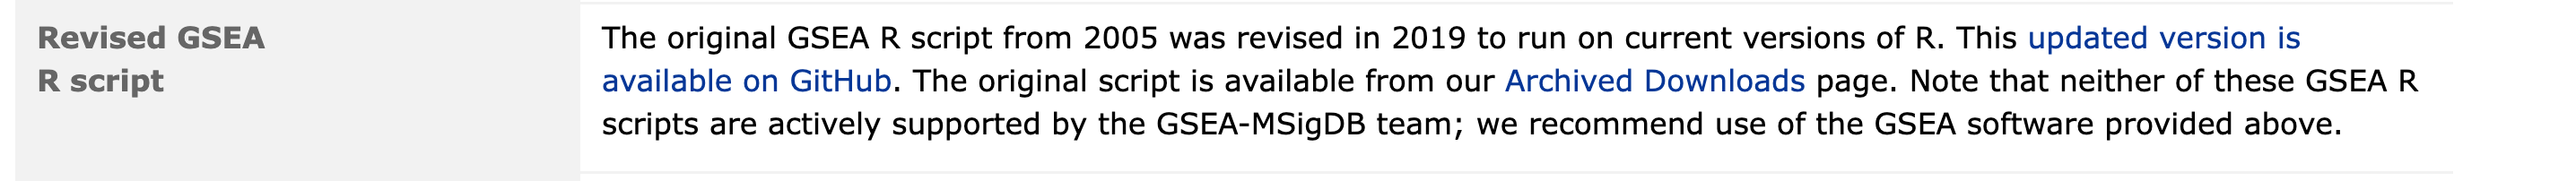
\includegraphics{./images/gsea_r_package_message.png}

\hypertarget{load-in-required-libraries}{%
\section{Load in required libraries}\label{load-in-required-libraries}}

\begin{Shaded}
\begin{Highlighting}[]
\CommentTok{\#install required R and bioconductor packages}
\FunctionTok{tryCatch}\NormalTok{(}\AttributeTok{expr =}\NormalTok{ \{ }\FunctionTok{library}\NormalTok{(}\StringTok{"RCurl"}\NormalTok{)\}, }
         \AttributeTok{error =} \ControlFlowTok{function}\NormalTok{(e) \{  }
           \FunctionTok{install.packages}\NormalTok{(}\StringTok{"RCurl"}\NormalTok{)\}, }
         \AttributeTok{finally =} \FunctionTok{library}\NormalTok{(}\StringTok{"RCurl"}\NormalTok{))}
\end{Highlighting}
\end{Shaded}

\hypertarget{configurable-parameters}{%
\section{Configurable Parameters}\label{configurable-parameters}}

In order to run GSEA automatically through the notebook you will need to download the gsea jar from \href{http://software.broadinstitute.org/gsea/downloads.jsp}{here}. Specify the exact path to the gsea jar in the parameters in order to automatically compute enrichments using GSEA.

If you are running this notebook using the \href{https://hub.docker.com/r/risserlin/workshop_base_image}{baderlab workshop docker image} then the image comes pre-installed with the gsea jar that you can use to run gsea directly in the docker. The path to the GSEA jar in the docker is - /home/rstudio/GSEA\_4.3.2/gsea-cli.sh

In order to run GSEA automatically you need to speciry the path to the gsea jar file.
The gsea\_jar needs to be the full path to the GSEA 4.3.2 directory that you downloaded from GSEA. for example /Users/johnsmith/GSEA\_4.3.2/gsea-cli.sh

The parameters are set manually here but if you want to run the script from the command line then you can update the notebook to pull the parameters from the command line given arguments by updating each variable below to pull the values from the paramters - for example:

\begin{itemize}
\tightlist
\item
  variable \textless- params\$parameter\_name
\end{itemize}

For more details see - \href{https://bookdown.org/yihui/rmarkdown/params-declare.html}{defining and using parameters} and \href{https://bookdown.org/yihui/rmarkdown/params-knit.html}{Knitting with parameters}

\begin{Shaded}
\begin{Highlighting}[]
\CommentTok{\#path to GSEA jar }
\NormalTok{gsea\_jar }\OtherTok{\textless{}{-}} \StringTok{"/home/rstudio/GSEA\_4.3.2/gsea{-}cli.sh"}
\end{Highlighting}
\end{Shaded}

Set the working directory as the directory to the directory where you downloaded all protocol files. For example /User/JohnSmith/EMProtocolFiles/data

\begin{Shaded}
\begin{Highlighting}[]
\CommentTok{\#directory where all the data files are found.  For example {-}   ./data/ }
\NormalTok{working\_dir }\OtherTok{\textless{}{-}} \StringTok{"./data/"}

\CommentTok{\#The name to give the analysis in GSEA {-} for example Mesen\_vs\_Immuno}
\NormalTok{analysis\_name }\OtherTok{\textless{}{-}} \StringTok{"Mesen\_vs\_Immuno"}

\CommentTok{\#rank file to use in GSEA analysis.  }
\CommentTok{\#For example {-} MesenchymalvsImmunoreactive\_edger\_ranks.rnk}
\NormalTok{rnk\_file }\OtherTok{\textless{}{-}} \StringTok{"MesenchymalvsImmunoreactive\_edger\_ranks.rnk"}

\CommentTok{\#run\_gsea {-} true/false}
\CommentTok{\# This parameter is for the compilation of the notebook.  }
\NormalTok{run\_gsea }\OtherTok{\textless{}{-}} \ConstantTok{FALSE}
\end{Highlighting}
\end{Shaded}

\hypertarget{download-the-latest-pathway-definition-file}{%
\section{Download the latest pathway definition file}\label{download-the-latest-pathway-definition-file}}

Only Human, Mouse, Rat, and Woodchuck gene set files are currently available on the baderlab downloads site. If you are working with a species other than human (and it is either rat,mouse or woodchuck) change the gmt\_url below to the correct species. Check \href{http://download.baderlab.org/EM_Genesets/current_release/}{here} to see all available species.

To create your own GMT file using Ensembl see \protect\hyperlink{create-gmt-file-from-ensembl}{Create GMT file from Ensembl}

\begin{Shaded}
\begin{Highlighting}[]
\NormalTok{gmt\_url }\OtherTok{=} \StringTok{"http://download.baderlab.org/EM\_Genesets/current\_release/Human/symbol/"}

\CommentTok{\#list all the files on the server}
\NormalTok{filenames }\OtherTok{=} \FunctionTok{getURL}\NormalTok{(gmt\_url)}
\NormalTok{tc }\OtherTok{=} \FunctionTok{textConnection}\NormalTok{(filenames)}
\NormalTok{contents }\OtherTok{=} \FunctionTok{readLines}\NormalTok{(tc)}
\FunctionTok{close}\NormalTok{(tc)}

\CommentTok{\#get the gmt that has all the pathways and does not include terms }
\CommentTok{\# inferred from electronic annotations(IEA)}
\CommentTok{\#start with gmt file that has pathways only and GO Biological Process only.}
\NormalTok{rx }\OtherTok{=} \FunctionTok{gregexpr}\NormalTok{(}\StringTok{"(?\textless{}=\textless{}a href=}\SpecialCharTok{\textbackslash{}"}\StringTok{)(.*.GOBP\_AllPathways\_no\_GO\_iea.*.)(.gmt)(?=}\SpecialCharTok{\textbackslash{}"}\StringTok{\textgreater{})"}\NormalTok{,}
\NormalTok{  contents, }\AttributeTok{perl =} \ConstantTok{TRUE}\NormalTok{)}
\NormalTok{gmt\_file }\OtherTok{=} \FunctionTok{unlist}\NormalTok{(}\FunctionTok{regmatches}\NormalTok{(contents, rx))}

\NormalTok{dest\_gmt\_file }\OtherTok{\textless{}{-}} \FunctionTok{file.path}\NormalTok{(working\_dir,gmt\_file )}

\CommentTok{\#check if this gmt file already exists}
\ControlFlowTok{if}\NormalTok{(}\SpecialCharTok{!}\FunctionTok{file.exists}\NormalTok{(dest\_gmt\_file))\{}
  \FunctionTok{download.file}\NormalTok{(}
    \FunctionTok{paste}\NormalTok{(gmt\_url,gmt\_file,}\AttributeTok{sep=}\StringTok{""}\NormalTok{),}
    \AttributeTok{destfile=}\NormalTok{dest\_gmt\_file}
\NormalTok{  )}
\NormalTok{\}}
\end{Highlighting}
\end{Shaded}

\begin{center}\rule{0.5\linewidth}{0.5pt}\end{center}

\hypertarget{run-gsea}{%
\section{Run GSEA}\label{run-gsea}}

(GSEA){[}\url{http://software.broadinstitute.org/gsea/index.jsp}{]} is a stand alone java program with many customizable options. It can be easily run through its integrated user interface. To make this a seemless pipeline we can run GSEA from the command line with a set of options. Any of the supplied options can be customized and there are many additional options that can be specified. For more details see (here){[}\url{http://software.broadinstitute.org/gsea/doc/GSEAUserGuideTEXT.htm\#_Running_GSEA_from}{]}

In the below command the following options have been specified:

\begin{itemize}
\tightlist
\item
  rnk - path to the rank file
\item
  gmx - path to the gene set definition (gmt) file
\item
  collapse - true/false indicates whether the expression/rnk file needs to be collapsed from probes to gene symbols
\item
  nperm - number of permutations
\item
  scoring\_scheme -
\item
  rpt\_label - name of the directory with output
\item
  rnd\_seed - random seed to use
\item
  set\_max - maximum size for individual gene sets. In GSEA interface this is set to 500 but we prefer to use a more stringent setting of 200.
\item
  set\_min - minimum size for individual gene sets
\item
  zip\_report - true/false to zip output directory
\item
  out - directory where to place the result directory.
\end{itemize}

\begin{Shaded}
\begin{Highlighting}[]
\ControlFlowTok{if}\NormalTok{(run\_gsea)\{}
\NormalTok{  command }\OtherTok{\textless{}{-}} \FunctionTok{paste}\NormalTok{(}\StringTok{""}\NormalTok{,gsea\_jar,  }
                   \StringTok{"GSEAPreRanked {-}gmx"}\NormalTok{, dest\_gmt\_file, }
                   \StringTok{"{-}rnk"}\NormalTok{ ,}\FunctionTok{file.path}\NormalTok{(working\_dir,rnk\_file), }
                   \StringTok{"{-}collapse false {-}nperm 1000 {-}scoring\_scheme weighted"}\NormalTok{, }
                   \StringTok{"{-}rpt\_label "}\NormalTok{,analysis\_name,}
                   \StringTok{"  {-}plot\_top\_x 20 {-}rnd\_seed 12345  {-}set\_max 200"}\NormalTok{,  }
                   \StringTok{" {-}set\_min 15 {-}zip\_report false "}\NormalTok{,}
                   \StringTok{" {-}out"}\NormalTok{ ,working\_dir, }
                   \StringTok{" \textgreater{} gsea\_output.txt"}\NormalTok{,}\AttributeTok{sep=}\StringTok{" "}\NormalTok{)}
  \FunctionTok{system}\NormalTok{(command)}
\NormalTok{\}}
\end{Highlighting}
\end{Shaded}

\hypertarget{create-gmt-file-from-ensembl}{%
\chapter{Create GMT file from Ensembl}\label{create-gmt-file-from-ensembl}}

The \href{https://download.baderlab.org/EM_Genesets/}{Baderlab geneset download site} is an updated resource for geneset files from GO, Reactome, WikiPathways, Pathbank, NetPath, HumanCyc, IOB, \ldots{} many others that can be used in \href{https://biit.cs.ut.ee/gprofiler/gost}{g:Profiler} or \href{https://www.gsea-msigdb.org/gsea/index.jsp}{GSEA} and many other enrichment tools that support the gmt format.

Unfortunately genesets are only supplied for:

\begin{itemize}
\tightlist
\item
  \href{https://download.baderlab.org/EM_Genesets/current_release/Human/}{Human}
\item
  \href{https://download.baderlab.org/EM_Genesets/current_release/Mouse/}{Mouse}
\item
  \href{https://download.baderlab.org/EM_Genesets/current_release/Rat/}{Rat}
\item
  \href{https://download.baderlab.org/EM_Genesets/current_release/Woodchuck/}{Woodchuck}
\end{itemize}

If you are working in a different species you will need to generate your own gmt file. The best way to do this is through ensembl. Ensembl doesn't have annotations for all the pathway databases listed above but it has annotations for most species from GO.

The parameters are set in the params option on this notebook but you can also manually set them here.

\begin{Shaded}
\begin{Highlighting}[]
\CommentTok{\# for example {-} working\_dir \textless{}{-} "./genereated\_data"}
\NormalTok{working\_dir }\OtherTok{\textless{}{-}}\NormalTok{ params}\SpecialCharTok{$}\NormalTok{working\_dir}

\CommentTok{\# for example {-} species \textless{}{-} "horse"}
\NormalTok{species }\OtherTok{\textless{}{-}}\NormalTok{ params}\SpecialCharTok{$}\NormalTok{species}

\CommentTok{\# for example {-} ensembl\_dataset \textless{}{-} "ecaballus\_gene\_ensembl"}
\NormalTok{ensembl\_dataset }\OtherTok{\textless{}{-}}\NormalTok{ params}\SpecialCharTok{$}\NormalTok{ensembl\_dataset}
\end{Highlighting}
\end{Shaded}

\begin{Shaded}
\begin{Highlighting}[]
\CommentTok{\#use library}
\CommentTok{\#make sure biocManager is installed}
\FunctionTok{tryCatch}\NormalTok{(}\AttributeTok{expr =}\NormalTok{ \{ }\FunctionTok{library}\NormalTok{(}\StringTok{"BiocManager"}\NormalTok{)\}, }
         \AttributeTok{error =} \ControlFlowTok{function}\NormalTok{(e) \{ }
           \FunctionTok{install.packages}\NormalTok{(}\StringTok{"BiocManager"}\NormalTok{)\}, }
         \AttributeTok{finally =} \FunctionTok{library}\NormalTok{(}\StringTok{"BiocManager"}\NormalTok{))}


\FunctionTok{tryCatch}\NormalTok{(}\AttributeTok{expr =}\NormalTok{ \{ }\FunctionTok{library}\NormalTok{(}\StringTok{"biomaRt"}\NormalTok{)\}, }
         \AttributeTok{error =} \ControlFlowTok{function}\NormalTok{(e) \{ }
\NormalTok{           BiocManager}\SpecialCharTok{::}\FunctionTok{install}\NormalTok{(}\StringTok{"biomaRt"}\NormalTok{)\}, }
         \AttributeTok{finally =} \FunctionTok{library}\NormalTok{(}\StringTok{"biomaRt"}\NormalTok{))}
\end{Highlighting}
\end{Shaded}

\hypertarget{load-libraries}{%
\section{Load Libraries}\label{load-libraries}}

Create or set a directory to store all the generatd results

\begin{Shaded}
\begin{Highlighting}[]
\ControlFlowTok{if}\NormalTok{(}\SpecialCharTok{!}\FunctionTok{dir.exists}\NormalTok{(params}\SpecialCharTok{$}\NormalTok{working\_dir))\{}
  \FunctionTok{dir.create}\NormalTok{(params}\SpecialCharTok{$}\NormalTok{working\_dir)}
\NormalTok{\}}
\end{Highlighting}
\end{Shaded}

\hypertarget{set-up-biomart-connection}{%
\section{Set up Biomart connection}\label{set-up-biomart-connection}}

Connect to Biomart

\begin{Shaded}
\begin{Highlighting}[]
\NormalTok{ensembl }\OtherTok{\textless{}{-}} \FunctionTok{useMart}\NormalTok{(}\StringTok{"ensembl"}\NormalTok{)}
\end{Highlighting}
\end{Shaded}

Figure out which dataset you want to use - for some species there might be a few datasets to choose from. Not all of the datasets have common namesa associated with them. For example, if you search for `yeast' nothing will be returned but if you look for Saccharomyces or cerevisiae you will be able to find it.

\begin{Shaded}
\begin{Highlighting}[]
\NormalTok{all\_datasets }\OtherTok{\textless{}{-}} \FunctionTok{listDatasets}\NormalTok{(ensembl)}

\CommentTok{\#get all the datasets that match our species definition}
\NormalTok{all\_datasets[}\FunctionTok{grep}\NormalTok{(all\_datasets}\SpecialCharTok{$}\NormalTok{description,}
                  \AttributeTok{pattern=}\NormalTok{species,}
                  \AttributeTok{ignore.case =} \ConstantTok{TRUE}\NormalTok{),]}
\end{Highlighting}
\end{Shaded}

\begin{verbatim}
##                         dataset                                 description
## 60       ecaballus_gene_ensembl                     Horse genes (EquCab3.0)
## 76          hcomes_gene_ensembl  Tiger tail seahorse genes (H_comes_QL1_v1)
## 164 rferrumequinum_gene_ensembl Greater horseshoe bat genes (mRhiFer1_v1.p)
##            version
## 60       EquCab3.0
## 76  H_comes_QL1_v1
## 164  mRhiFer1_v1.p
\end{verbatim}

If you know the ensembl dataset that you want to use you can specify it in the parameters above or grab from the above table the dataset of the species that you are interested in.

\begin{Shaded}
\begin{Highlighting}[]
\NormalTok{ensembl }\OtherTok{=} \FunctionTok{useDataset}\NormalTok{(ensembl\_dataset,}\AttributeTok{mart=}\NormalTok{ensembl)}
\end{Highlighting}
\end{Shaded}

\hypertarget{get-species-go-annotations}{%
\section{Get species GO annotations}\label{get-species-go-annotations}}

Get the GO annotations for our species

\begin{Shaded}
\begin{Highlighting}[]
\NormalTok{go\_annotation }\OtherTok{\textless{}{-}} \FunctionTok{getBM}\NormalTok{(}\AttributeTok{attributes =} \FunctionTok{c}\NormalTok{(}\StringTok{"external\_gene\_name"}\NormalTok{,}
                                      \StringTok{"ensembl\_gene\_id"}\NormalTok{,}
                                      \StringTok{"ensembl\_transcript\_id"}\NormalTok{,}
                                      \StringTok{"go\_id"}\NormalTok{, }
                                      \StringTok{"name\_1006"}\NormalTok{, }
                                      \StringTok{"namespace\_1003"}\NormalTok{,}
                                      \StringTok{"go\_linkage\_type"}\NormalTok{), }
                       \AttributeTok{filters=}\FunctionTok{list}\NormalTok{(}\AttributeTok{biotype=}\StringTok{\textquotesingle{}protein\_coding\textquotesingle{}}\NormalTok{), }\AttributeTok{mart=}\NormalTok{ensembl);}

\CommentTok{\#get just the go biological process subset}
\DocumentationTok{\#\#\#\#\#}
\CommentTok{\# Get rid of this line if you want to include all of go and not just biological process}
\DocumentationTok{\#\#\#\#\#}
\NormalTok{go\_annotation\_bp }\OtherTok{\textless{}{-}}\NormalTok{ go\_annotation[}\FunctionTok{which}\NormalTok{(}
\NormalTok{  go\_annotation}\SpecialCharTok{$}\NormalTok{namespace\_1003 }\SpecialCharTok{==} \StringTok{"biological\_process"}\NormalTok{),]}

\CommentTok{\#compute the unique pathway sets}
\NormalTok{go\_pathway\_sets }\OtherTok{\textless{}{-}} \FunctionTok{aggregate}\NormalTok{(go\_annotation\_bp[,}\DecValTok{1}\SpecialCharTok{:}\DecValTok{5}\NormalTok{],}
                             \AttributeTok{by =} \FunctionTok{list}\NormalTok{(go\_annotation\_bp}\SpecialCharTok{$}\NormalTok{go\_id),}
                             \AttributeTok{FUN =} \ControlFlowTok{function}\NormalTok{(x)\{}\FunctionTok{list}\NormalTok{(}\FunctionTok{unique}\NormalTok{(x))\})}

\CommentTok{\#unlist the go descriptions}
\NormalTok{go\_pathway\_sets}\SpecialCharTok{$}\NormalTok{name\_1006 }\OtherTok{\textless{}{-}} \FunctionTok{apply}\NormalTok{(go\_pathway\_sets,}\DecValTok{1}\NormalTok{,}\AttributeTok{FUN=}\ControlFlowTok{function}\NormalTok{(x)\{}
   \FunctionTok{paste}\NormalTok{(}\FunctionTok{gsub}\NormalTok{(}\FunctionTok{unlist}\NormalTok{(x}\SpecialCharTok{$}\NormalTok{name\_1006),}\AttributeTok{pattern=} \StringTok{"}\SpecialCharTok{\textbackslash{}"}\StringTok{"}\NormalTok{,}
              \AttributeTok{replacement =} \StringTok{""}\NormalTok{),}\AttributeTok{collapse =} \StringTok{""}\NormalTok{)\})}
\end{Highlighting}
\end{Shaded}

There are two identifiers that you can choose from in the above table
* external\_symbols
* ensembl\_ids

Each of these is stored as a list in the dataframe. In order to convert it to the right format for the gmt file we need to convert the list to string of tab delimited strings. (unfortunately there is no streaightforward way to write out a dataframe's column of lists.)

\begin{Shaded}
\begin{Highlighting}[]
\NormalTok{go\_pathway\_sets[}\DecValTok{1}\SpecialCharTok{:}\DecValTok{3}\NormalTok{,}\StringTok{"external\_gene\_name"}\NormalTok{]}
\end{Highlighting}
\end{Shaded}

\begin{verbatim}
## [[1]]
## [1] "MEF2A"    "SLC25A36" "OPA1"     "MGME1"    "SLC25A33" "TYMP"     "AKT3"    
## [8] "PIF1"    
## 
## [[2]]
## [1] "GNRH1" "GNRH2" "LIN9" 
## 
## [[3]]
## [1] "ERCC6" "ERCC8" "LIG4"  "APLF"  "APTX"  "XRCC1" "SIRT1" "XNDC1"
\end{verbatim}

\begin{Shaded}
\begin{Highlighting}[]
\NormalTok{go\_pathway\_sets[}\DecValTok{1}\SpecialCharTok{:}\DecValTok{3}\NormalTok{,}\StringTok{"ensembl\_gene\_id"}\NormalTok{]}
\end{Highlighting}
\end{Shaded}

\begin{verbatim}
## [[1]]
## [1] "ENSECAG00000011593" "ENSECAG00000010094" "ENSECAG00000024248"
## [4] "ENSECAG00000012675" "ENSECAG00000016862" "ENSECAG00000001072"
## [7] "ENSECAG00000019722" "ENSECAG00000005316"
## 
## [[2]]
## [1] "ENSECAG00000010664" "ENSECAG00000039220" "ENSECAG00000014325"
## 
## [[3]]
## [1] "ENSECAG00000014160" "ENSECAG00000018335" "ENSECAG00000003257"
## [4] "ENSECAG00000013246" "ENSECAG00000012674" "ENSECAG00000014127"
## [7] "ENSECAG00000013909" "ENSECAG00000042118"
\end{verbatim}

\hypertarget{format-results-into-gmt-file}{%
\section{Format results into GMT file}\label{format-results-into-gmt-file}}

Convert column of lists to a tab delimited string of gene names

\begin{Shaded}
\begin{Highlighting}[]
\NormalTok{go\_pathway\_sets}\SpecialCharTok{$}\NormalTok{collapsed\_genenames }\OtherTok{\textless{}{-}} \FunctionTok{apply}\NormalTok{(go\_pathway\_sets,}\DecValTok{1}\NormalTok{,}
                                             \AttributeTok{FUN=}\ControlFlowTok{function}\NormalTok{(x)\{}
   \FunctionTok{paste}\NormalTok{(}\FunctionTok{gsub}\NormalTok{(}\FunctionTok{unlist}\NormalTok{(x}\SpecialCharTok{$}\NormalTok{external\_gene\_name),}\AttributeTok{pattern=} \StringTok{"}\SpecialCharTok{\textbackslash{}"}\StringTok{"}\NormalTok{,}
              \AttributeTok{replacement =} \StringTok{""}\NormalTok{),}\AttributeTok{collapse =} \StringTok{"}\SpecialCharTok{\textbackslash{}t}\StringTok{"}\NormalTok{)}
\NormalTok{\})}
\end{Highlighting}
\end{Shaded}

Convert column of lists to a tab delimited string of gene names

\begin{Shaded}
\begin{Highlighting}[]
\NormalTok{go\_pathway\_sets}\SpecialCharTok{$}\NormalTok{collapsed\_ensemblids }\OtherTok{\textless{}{-}} \FunctionTok{apply}\NormalTok{(go\_pathway\_sets,}\DecValTok{1}\NormalTok{,}
                                              \AttributeTok{FUN=}\ControlFlowTok{function}\NormalTok{(x)\{}
   \FunctionTok{paste}\NormalTok{(}\FunctionTok{gsub}\NormalTok{(}\FunctionTok{unlist}\NormalTok{(x}\SpecialCharTok{$}\NormalTok{ensembl\_gene\_id),}\AttributeTok{pattern=} \StringTok{"}\SpecialCharTok{\textbackslash{}"}\StringTok{"}\NormalTok{,}
              \AttributeTok{replacement =} \StringTok{""}\NormalTok{),}\AttributeTok{collapse =} \StringTok{"}\SpecialCharTok{\textbackslash{}t}\StringTok{"}\NormalTok{)}
\NormalTok{\})}
\end{Highlighting}
\end{Shaded}

The format of the GMT file is described \href{here}{https://software.broadinstitute.org/cancer/software/gsea/wiki/index.php/Data\_formats\#GMT:\emph{Gene\_Matrix\_Transposed\_file\_format}.28.2A.gmt.29} and consists of rows with the following

\begin{itemize}
\tightlist
\item
  Name
\item
  Description
\item
  tab delimited list of genes a part of this geneset
\end{itemize}

Write out the gmt file with genenames

\begin{Shaded}
\begin{Highlighting}[]
\NormalTok{gmt\_file\_genenames }\OtherTok{\textless{}{-}}\NormalTok{ go\_pathway\_sets[,}\FunctionTok{c}\NormalTok{(}\StringTok{"Group.1"}\NormalTok{,}\StringTok{"name\_1006"}\NormalTok{,}
                                         \StringTok{"collapsed\_genenames"}\NormalTok{)]}
\FunctionTok{colnames}\NormalTok{(gmt\_file\_genenames)[}\DecValTok{1}\SpecialCharTok{:}\DecValTok{2}\NormalTok{] }\OtherTok{\textless{}{-}} \FunctionTok{c}\NormalTok{(}\StringTok{"name"}\NormalTok{,}\StringTok{"description"}\NormalTok{) }

\NormalTok{gmt\_genenames\_filename }\OtherTok{\textless{}{-}} \FunctionTok{file.path}\NormalTok{(params}\SpecialCharTok{$}\NormalTok{working\_dir, }\FunctionTok{paste}\NormalTok{(species,ensembl\_dataset,}\StringTok{"GO\_genesets\_GN.gmt"}\NormalTok{,}\AttributeTok{sep =} \StringTok{"\_"}\NormalTok{))}

\FunctionTok{write.table}\NormalTok{(}\AttributeTok{x =}\NormalTok{ gmt\_file\_genenames,}\AttributeTok{file =}\NormalTok{ gmt\_genenames\_filename,}
            \AttributeTok{quote =} \ConstantTok{FALSE}\NormalTok{,}\AttributeTok{sep =} \StringTok{"}\SpecialCharTok{\textbackslash{}t}\StringTok{"}\NormalTok{,}\AttributeTok{row.names =} \ConstantTok{FALSE}\NormalTok{,}
            \AttributeTok{col.names=}\ConstantTok{TRUE}\NormalTok{)}
\end{Highlighting}
\end{Shaded}

Write out the gmt file with ensembl ids

\begin{Shaded}
\begin{Highlighting}[]
\NormalTok{gmt\_file\_ensemblids }\OtherTok{\textless{}{-}}\NormalTok{ go\_pathway\_sets[,}\FunctionTok{c}\NormalTok{(}\StringTok{"Group.1"}\NormalTok{,}\StringTok{"name\_1006"}\NormalTok{,}
                                          \StringTok{"collapsed\_ensemblids"}\NormalTok{)]}
\FunctionTok{colnames}\NormalTok{(gmt\_file\_ensemblids)[}\DecValTok{1}\SpecialCharTok{:}\DecValTok{2}\NormalTok{] }\OtherTok{\textless{}{-}} \FunctionTok{c}\NormalTok{(}\StringTok{"name"}\NormalTok{,}\StringTok{"description"}\NormalTok{) }

\NormalTok{gmt\_ensemblids\_filename }\OtherTok{\textless{}{-}} \FunctionTok{file.path}\NormalTok{(params}\SpecialCharTok{$}\NormalTok{working\_dir, }\FunctionTok{paste}\NormalTok{(species,ensembl\_dataset,}\StringTok{"GO\_genesets\_esemblids.gmt"}\NormalTok{,}\AttributeTok{sep =} \StringTok{"\_"}\NormalTok{))}

\FunctionTok{write.table}\NormalTok{(}\AttributeTok{x =}\NormalTok{ gmt\_file\_ensemblids,}\AttributeTok{file =}\NormalTok{ gmt\_ensemblids\_filename,}
            \AttributeTok{quote =} \ConstantTok{FALSE}\NormalTok{,}\AttributeTok{sep =} \StringTok{"}\SpecialCharTok{\textbackslash{}t}\StringTok{"}\NormalTok{,}\AttributeTok{row.names =} \ConstantTok{FALSE}\NormalTok{,}
            \AttributeTok{col.names=}\ConstantTok{TRUE}\NormalTok{)}
\end{Highlighting}
\end{Shaded}

\hypertarget{refs}{}
\begin{CSLReferences}{1}{0}
\leavevmode\vadjust pre{\hypertarget{ref-em2019}{}}%
Reimand, Jüri, Ruth Isserlin, Veronique Voisin, Mike Kucera, Christian Tannus-Lopes, Asha Rostamianfar, Lina Wadi, et al. 2019. {``Pathway Enrichment Analysis and Visualization of Omics Data Using g: Profiler, GSEA, Cytoscape and EnrichmentMap.''} \emph{Nature Protocols} 14 (2): 482--517.

\leavevmode\vadjust pre{\hypertarget{ref-gsea2005}{}}%
Subramanian, Aravind, Pablo Tamayo, Vamsi K Mootha, Sayan Mukherjee, Benjamin L Ebert, Michael A Gillette, Amanda Paulovich, et al. 2005. {``Gene Set Enrichment Analysis: A Knowledge-Based Approach for Interpreting Genome-Wide Expression Profiles.''} \emph{Proceedings of the National Academy of Sciences} 102 (43): 15545--50.

\leavevmode\vadjust pre{\hypertarget{ref-docker}{}}%
{``What Is a Container?''} n.d. \emph{Docker}. \url{https://www.docker.com/resources/what-container}.

\leavevmode\vadjust pre{\hypertarget{ref-xie2015}{}}%
Xie, Yihui. 2015. \emph{Dynamic Documents with {R} and Knitr}. 2nd ed. Boca Raton, Florida: Chapman; Hall/CRC. \url{http://yihui.name/knitr/}.

\leavevmode\vadjust pre{\hypertarget{ref-R-bookdown}{}}%
---------. 2023. \emph{Bookdown: Authoring Books and Technical Documents with r Markdown}. \url{https://CRAN.R-project.org/package=bookdown}.

\end{CSLReferences}

\end{document}
